%%%%%%%%%%%%%%%%%%%%%%%%%%%%%%%%%%%%%%%%%%%%%%%%%%%%%%%%%%%%%%%%%%%%%%%%%
%  Zawartość: Główny plik szablonu pracy dyplomowej (magisterskiej/inżynierskiej).
%  Opracował: Tomasz Kubik <tomasz.kubik@pwr.edu.pl>
%  Data: 1 marca 2020
%  Wersja: 0.4
%%%%%%%%%%%%%%%%%%%%%%%%%%%%%%%%%%%%%%%%%%%%%%%%%%%%%%%%%%%%%%%%%%%%%%%%%

\documentclass[a4paper,onecolumn,oneside,12pt,extrafontsizes]{memoir}
% W celu przygotowania wydruku  do archiwum można:
% a) przygotować pdf, w którym dwie strony zostaną wstawione na jedną fizyczną stronę i taki dokument wydrukować dwustronnie (podejście zalecane)
%
%   Taki dokument można przygotować poprzez
%   - wydruk z Adobe Acrobat Reader z opcją "Wiele" - sekcja "Rozmiar i obsługa stron"
%   - wykorzystanie narzędzi psutils
%
%      Windows (zakładając, że w dystrybucji MiKTeX jest pakiet miktex-psutils-bin-x64-2.9):
%        "c:\Program Files\MiKTeX 2.9\miktex\bin\x64\pdf2ps.exe" Dyplom.pdf Dyplom.ps
%        "c:\Program Files\MiKTeX 2.9\miktex\bin\x64\psnup.exe" -2 Dyplom.ps Dyplom2.ps
%        "c:\Program Files\MiKTeX 2.9\miktex\bin\x64\ps2pdf.exe" Dyplom2.ps Dyplom2.pdf
%        Del Dyplom2.ps Dyplom.ps
%
%     Linux:
%        pdf2ps Dyplom.pdf - | psnup -2 | ps2pdf - Dyplom2.pdf
%
%
% b) przekomplilować dokument zmniejszając czcionkę (podejście niezalecane, bo zmienia formatowanie dokumentu)
%
%    Do tego wystarczy posłużyć się dwoma poniższymi komendami (zamiast documentclass z pierwszej linijki):
%   \documentclass[a4paper,onecolumn,twoside,10pt]{memoir} 
%   \renewcommand{\normalsize}{\fontsize{8pt}{10pt}\selectfont}

%\usepackage[cp1250]{inputenc} % jeśli kodowanie edytowanych plików to cp1250 
\usepackage[utf8]{inputenc} % jeśli kodowanie edytowanych plików to UTF8
\usepackage[T1]{fontenc}
\usepackage[polish]{babel}
%\DisemulatePackage{setspace}
\usepackage{setspace}
\usepackage{tabularx}
\usepackage{color,calc}
%\usepackage{soul} % pakiet z komendami do podkreślania tekstu

\usepackage{ebgaramond} % pakiet z czcionkami garamond, potrzebny tylko do strony tytułowej, musi wystąpić przed pakietem tgtermes

%% Aby uzyskać polskie literki w pdfie (a nie zlepki) korzystamy z pakietu czcionek tgterms. 
%% W pakiecie tym są zdefiniowane klony czcionek Times o kształtach: normalny, pogrubiony, italic, italic pogrubiony.
%% W pakiecie tym brakuje czcionki o kształcie: slanted (podobny do italic). 
%% Jeśli w dokumencie gdzieś zostanie zastosowana czcionka slanted (np. po użyciu komendy \textsl{}), to
%% latex dokona podstawienia na czcionkę standardową i zgłosi to w ostrzeżeniu (warningu).
%% Ponadto tgtermes to czcionka do tekstu. Wszelkie matematyczne wzory będą sformatowane domyślną czcionką do wzorów.
%% Jeśli wzory mają być sformatowane z wykorzystaniem innych czcionek, trzeba to jawnie zadeklarować.

%% BĄCZKOWE BIBLIOTEKI

\usepackage{tikz}
\usetikzlibrary{er,positioning}

\usepackage[edges]{forest}
\forestset{
  direction switch/.style={
    for tree={edge+=thick, font=\sffamily},
    where level>=1{folder, grow'=0}{for children=forked edge},
    where level=3{}{draw},
  },
}

\usepackage{float}
\usepackage{multicol}
% \usepackage{lscape}
% we want ER + above/below + left/right

%% END OF BĄCZKOWE BIBLIOTEKI

%% Po zainstalowaniu pakietu tgtermes może będzie trzeba zauktualizować informacje 
%% o dostępnych fontach oraz mapy. Można to zrobić z konsoli (jako administrator)
%% initexmf --admin --update-fndb
%% initexmf --admin --mkmaps

\usepackage{tgtermes}   
\renewcommand*\ttdefault{txtt}

% We wcześniejszej wersji szablonu korzystano z innych czcionek. Dla celów historycznych pozostawiono je w komentarzu
%\usepackage{mathptmx} % pakiet będący następcą pakietów times and mathptm, niestety polskie literki są zlepkami
%\usepackage{newtxtext,newtxmath} % pakiety dostarczające Times dla tekstów i wzorów matematycznych,  
%                                  rozwiązuje problemy występujące w mathptmx, ale wymaga zainstalowania
%                                  dodatkowych pakietów oraz uruchomienia updmap (konsola administratora)
%                                  niestety polskie literki są zlepkami
%\usepackage{newtxmath,tgtermes} % można też połączyć czcionki do tekstu i czcionki do wzorów

\usepackage{listings} % pakiet do prezentacji kodu. 
% Wcześniej był problem z polskimi znakami w otoczeniu lstlisting, stąd poniższe rozwiązanie: 
\lstset{literate=%-
{ą}{{\k{a}}}1 {ć}{{\'c}}1 {ę}{{\k{e}}}1 {ł}{{\l{}}}1 {ń}{{\'n}}1 {ó}{{\'o}}1 {ś}{{\'s}}1 {ż}{{\.z}}1 {ź}{{\'z}}1 {Ą}{{\k{A}}}1 {Ć}{{\'C}}1 {Ę}{{\k{E}}}1 {Ł}{{\L{}}}1 {Ń}{{\'N}}1 {Ó}{{\'O}}1 {Ś}{{\'S}}1 {Ż}{{\.Z}}1 {Ź}{{\'Z}}1 
    {Ö}{{\"O}}1
    {Ä}{{\"A}}1
    {Ü}{{\"U}}1
    {ß}{{\ss}}1
    {ü}{{\"u}}1
    {ä}{{\"a}}1
    {ö}{{\"o}}1
    {~}{{\textasciitilde}}1
		{—}{{{\textemdash} }}1
}%{\ \ }{{\ }}1}


\newcommand{\listingcaption}[1]% dodane, by można było robić podpis nad dwukolumnowym listingiem
{%
\vspace*{\abovecaptionskip}\small 
\refstepcounter{lstlisting}\hfill%
Listing \thelstlisting: #1\hfill%\hfill%
\addcontentsline{lol}{lstlisting}{\protect\numberline{\thelstlisting}#1}
}%

% Styl zapewniający numerowanie linii
\lstset{
  %%basicstyle=\footnotesize\ttfamily,
  %%columns=fullflexible,
	%%showstringspaces=false,
	%%showspaces=false,
  breaklines=true,
  postbreak=\mbox{\textcolor{red}{$\hookrightarrow$}\space},
  %%numbers=left,
  %%firstnumber=1,
  %%numberfirstline=true,
	%%xleftmargin=17pt,
  %%framexleftmargin=17pt,
  %%framexrightmargin=5pt,
  %%framexbottommargin=4pt,
	belowskip=.5\baselineskip
}

% Styl bez numerownia linii
%%\lstset{
  %%basicstyle=\footnotesize\ttfamily,
  %%columns=fullflexible,
	%%showstringspaces=false,
	%%showspaces=false,
  %%breaklines=true,
  %%postbreak=\mbox{\textcolor{red}{$\hookrightarrow$}\space},
%%}

%% Poniżej sposób ostylowania sposobu podświetlania składni wybranych języków
%%\lstloadlanguages{% Check Dokumentation for further languages ...
%%C,
%%C++,
%%csh,
%%Java
%%}
%%
%%\definecolor{red}{rgb}{0.6,0,0} % for strings
%%\definecolor{blue}{rgb}{0,0,0.6}
%%\definecolor{green}{rgb}{0,0.8,0}
%%\definecolor{cyan}{rgb}{0.0,0.6,0.6}
%%
%%\lstdefinestyle{sqlstyle}{
%%language=SQL,
%%basicstyle=\footnotesize\ttfamily, 
%%numbers=left, 
%%numberstyle=\tiny, 
%%numbersep=5pt, 
%%tabsize=2, 
%%extendedchars=true, 
%%breaklines=true, 
%%showspaces=false, 
%%showtabs=true, 
%%xleftmargin=17pt,
%%framexleftmargin=17pt,
%%framexrightmargin=5pt,
%%framexbottommargin=4pt,
%%keywordstyle=\color{blue}, 
%%commentstyle=\color{green}, 
%%stringstyle=\color{red}, 
%%}
%%
%%\lstdefinestyle{sharpcstyle}{
%%language=[Sharp]C,
%%basicstyle=\footnotesize\ttfamily, 
%%numbers=left, 
%%numberstyle=\tiny, 
%%numbersep=5pt, 
%%tabsize=2, 
%%extendedchars=true, 
%%breaklines=true, 
%%showspaces=false, 
%%showtabs=true, 
%%xleftmargin=17pt,
%%framexleftmargin=17pt,
%%framexrightmargin=5pt,
%%framexbottommargin=4pt,
%%morecomment=[l]{//}, %use comment-line-style!
%%morecomment=[s]{/*}{*/}, %for multiline comments
%%showstringspaces=false, 
%%morekeywords={  abstract, event, new, struct,
                %%as, explicit, null, switch,
                %%base, extern, object, this,
                %%bool, false, operator, throw,
                %%break, finally, out, true,
                %%byte, fixed, override, try,
                %%case, float, params, typeof,
                %%catch, for, private, uint,
                %%char, foreach, protected, ulong,
                %%checked, goto, public, unchecked,
                %%class, if, readonly, unsafe,
                %%const, implicit, ref, ushort,
                %%continue, in, return, using,
                %%decimal, int, sbyte, virtual,
                %%default, interface, sealed, volatile,
                %%delegate, internal, short, void,
                %%do, is, sizeof, while,
                %%double, lock, stackalloc,
                %%else, long, static,
                %%enum, namespace, string},
%%keywordstyle=\color{cyan},
%%identifierstyle=\color{red},
%%stringstyle=\color{blue}, 
%%commentstyle=\color{green},
%%}

\renewcommand\lstlistlistingname{Spis listingów}
\makeatletter
%\renewcommand*{\l@lstlisting}[2]{\@dottedtocline{1}{0em}{2.3em}{#1}{#2}}
\g@addto@macro\insertchapterspace{\addtocontents{lol}{\protect\addvspace{10pt}}}
\renewcommand*{\l@lstlisting}{\@dottedtocline{1}{0em}{2.3em}}
\makeatother

\renewcommand*{\lstlistlistingname}{Spis listingów} \newlistof{lstlistoflistings}{lol}{\lstlistlistingname}



% Choć możliwe jest zastosowanie różnych pakietów formatujących tabele, zaleca się tego nie robić.
%\usepackage{longtable}
%\usepackage{ltxtable}
%\usepackage{tabulary}

%%%%%%%%%%%%%%%%%%%%%%%%%%%%%%%%%%%%%%%%%%%%%%%%%%%
%% Ustawienia odpowiedzialne za sposób łamania dokumentu
%% i ułożenie elementów pływających
%%%%%%%%%%%%%%%%%%%%%%%%%%%%%%%%%%%%%%%%%%%%%%%%%%%
%\hyphenpenalty=10000		% nie dziel wyrazów zbyt często
\clubpenalty=10000      %kara za sierotki
\widowpenalty=10000  % nie pozostawiaj wdów
%\brokenpenalty=10000		% nie dziel wyrazów między stronami - trzeba było wyłączyć, bo nie łamały się linie w lstlisting
%\exhyphenpenalty=999999		% nie dziel słów z myślnikiem - trzeba było wyłączyć, bo nie łamały się linie w lstlisting
\righthyphenmin=3			% dziel minimum 3 litery

%\tolerance=4500
%\pretolerance=250
%\hfuzz=1.5pt
%\hbadness=1450

\renewcommand{\topfraction}{0.95}
\renewcommand{\bottomfraction}{0.95}
\renewcommand{\textfraction}{0.05}
\renewcommand{\floatpagefraction}{0.35}

%%%%%%%%%%%%%%%%%%%%%%%%%%%%%%%%%%%%%%%%%%%%%%%%%%%
%%  Ustawienia rozmiarów: tekstu, nagłówka i stopki, marginesów
%%  dla dokumentów klasy memoir 
%%%%%%%%%%%%%%%%%%%%%%%%%%%%%%%%%%%%%%%%%%%%%%%%%%%
\setlength{\headsep}{10pt} 
\setlength{\headheight}{13.6pt} % wartość baselineskip dla czcionki 11pt tj. \small wynosi 13.6pt
\setlength{\footskip}{\headsep+\headheight}
\setlength{\uppermargin}{\headheight+\headsep+1cm}
\setlength{\textheight}{\paperheight-\uppermargin-\footskip-1.5cm}
\setlength{\textwidth}{\paperwidth-5cm}
\setlength{\spinemargin}{2.5cm}
\setlength{\foremargin}{2.5cm}
\setlength{\marginparsep}{2mm}
\setlength{\marginparwidth}{2.3mm}
%\settrimmedsize{297mm}{210mm}{*}
%\settrims{0mm}{0mm}	
\checkandfixthelayout[fixed] % konieczne, aby się dobrze wszystko poustawiało
%%%%%%%%%%%%%%%%%%%%%%%%%%%%%%%%%%%%%%%%%%%%%%%%
%%  Ustawienia odległości linii, wcięć, odstępów
%%%%%%%%%%%%%%%%%%%%%%%%%%%%%%%%%%%%%%%%%%%%%%%%
\linespread{1}
%\linespread{1.241}
\setlength{\parindent}{14.5pt}
%\setlength{\cftbeforechapterskip}{0.3em} % odstępy w spisie treści
%\setbeforesecskip{10pt plus 0.5ex}%{-3.5ex \@plus -1ex \@minus -.2ex}
%\setaftersecskip{10pt plus 0.5ex}%\onelineskip}
%\setbeforesubsecskip{8pt plus 0.5ex}%{-3.5ex \@plus -1ex \@minus -.2ex}
%\setaftersubsecskip{8pt plus 0.5ex}%\onelineskip}
%\setlength\floatsep{6pt plus 2pt minus 2pt} 
%\setlength\intextsep{12pt plus 2pt minus 2pt} 
%\setlength\textfloatsep{12pt plus 2pt minus 2pt} 

%%%%%%%%%%%%%%%%%%%%%%%%%%%%%%%%%%%%%%%%%%%%%%%%%%%
%%  Pakiety i komendy zastosowane tylko do zamieszczenia informacji o użytych komendach i fontach
%%  Normalnie nie są potrzebne, można je zamarkować podczas redakcji pracy
%%%%%%%%%%%%%%%%%%%%%%%%%%%%%%%%%%%%%%%%%%%%%%%%%%%
\usepackage{memlays}     % extra layout diagrams, zastosowane w szblonie do 'debuggowania', używa pakietu layouts
%\usepackage{layouts}
\usepackage{printlen} % pakiet do wyświetlania wartości zdefiniowanych długości, stosowany do 'debuggowania'
\uselengthunit{pt}
\makeatletter
\newcommand{\showFontSize}{\f@size pt} % makro wypisujące wielkość bieżącej czcionki
\makeatother
% do pokazania ramek można byłoby użyć:
%\usepackage{showframe} 


%%%%%%%%%%%%%%%%%%%%%%%%%%%%%%%%%%%%%%%%%%%%%%%%%%%
%%  Formatowanie list wyliczeniowych, wypunktowań i własnych otoczeń
%%%%%%%%%%%%%%%%%%%%%%%%%%%%%%%%%%%%%%%%%%%%%%%%%%%

% Domyślnie wypunktowania mają zadeklatorowane znaki, które nie występują w tgtermes
% Aby latex nie podstawiał w ich miejsca znaków z czcionki standardowej można zrobić podstawienie:
%    \DeclareTextCommandDefault{\textbullet}{\ensuremath{\bullet}}
%    \DeclareTextCommandDefault{\textasteriskcentered}{\ensuremath{\ast}}
%    \DeclareTextCommandDefault{\textperiodcentered}{\ensuremath{\cdot}}
% Jednak jeszcze lepszym pomysłem jest zdefiniowanie otoczeń z wykorzystaniem enumitem
\usepackage{enumitem} % pakiet pozwalający zarządzać formatowaniem list wyliczeniowych
\setlist{noitemsep,topsep=4pt,parsep=0pt,partopsep=4pt,leftmargin=*} % zadeklarowane parametry pozwalają uzyskać 'zwartą' postać wypunktowania bądź wyliczenia
\setenumerate{labelindent=0pt,itemindent=0pt,leftmargin=!,label=\arabic*.} % można zmienić \arabic na \alph, jeśli wyliczenia mają być z literkami
\setlistdepth{4} % definiujemy głębokość zagnieżdżenia list wyliczeniowych do 4 poziomów
\setlist[itemize,1]{label=$\bullet$}  % definiujemy, jaki symbol ma być użyty w wyliczeniu na danym poziomie
\setlist[itemize,2]{label=\normalfont\bfseries\textendash}
\setlist[itemize,3]{label=$\ast$}
\setlist[itemize,4]{label=$\cdot$}
\renewlist{itemize}{itemize}{4}

%%%http://tex.stackexchange.com/questions/29322/how-to-make-enumerate-items-align-at-left-margin
%\renewenvironment{enumerate}
%{
%\begin{list}{\arabic{enumi}.}
%{
%\usecounter{enumi}
%%\setlength{\itemindent}{0pt}
%%\setlength{\leftmargin}{1.8em}%{2zw} % 
%%\setlength{\rightmargin}{0zw} %
%%\setlength{\labelsep}{1zw} %
%%\setlength{\labelwidth}{3zw} % 
%\setlength{\topsep}{6pt}%
%\setlength{\partopsep}{0pt}%
%\setlength{\parskip}{0pt}%
%\setlength{\parsep}{0em} % 
%\setlength{\itemsep}{0em} % 
%%\setlength{\listparindent}{1zw} % 
%}
%}{
%\end{list}
%}

\makeatletter
\renewenvironment{quote}{
	\begin{list}{}
	{
	\setlength{\leftmargin}{1em}
	\setlength{\topsep}{0pt}%
	\setlength{\partopsep}{0pt}%
	\setlength{\parskip}{0pt}%
	\setlength{\parsep}{0pt}%
	\setlength{\itemsep}{0pt}
	}
	}{
	\end{list}}
\makeatother

%%%%%%%%%%%%%%%%%%%%%%%%%%%%%%%%%%%%%%%%%
%%  Pakiet do generowania indeksu (ważne, aby wstawić przed hyperref)
%%%%%%%%%%%%%%%%%%%%%%%%%%%%%%%%%%%%%%%%%
\DisemulatePackage{imakeidx}
\usepackage[makeindex,noautomatic]{imakeidx} % tutaj mówimy, żeby indeks nie generował się automatycznie, 

%\usepackage[noautomatic]{imakeidx} 
\makeindex

\makeatletter
%%%\renewenvironment{theindex}
							 %%%{\vskip 10pt\@makeschapterhead{\indexname}\vskip -3pt%
								%%%\@mkboth{\MakeUppercase\indexname}%
												%%%{\MakeUppercase\indexname}%
								%%%\vspace{-3.2mm}\parindent\z@%
								%%%\renewcommand\subitem{\par\hangindent 16\p@ \hspace*{0\p@}}%%
								%%%\phantomsection%
								%%%\begin{multicols}{2}
								%%%%\thispagestyle{plain}
								%%%\parindent\z@                
								%%%%\parskip\z@ \@plus .3\p@\relax
								%%%\let\item\@idxitem}
							 %%%{\end{multicols}\clearpage}
%%%
\makeatother


\usepackage{ifpdf}
%\newif\ifpdf \ifx\pdfoutput\undefined
%\pdffalse % we are not running PDFLaTeX
%\else
%\pdfoutput=1 % we are running PDFLaTeX
%\pdftrue \fi
\ifpdf
 \usepackage[pdftex,bookmarks,breaklinks,unicode]{hyperref}
%  WARNING - usunąłem to bo był jakiś "Option clash for package graphicx"   
%  \usepackage[pdftex]{graphicx}
 \DeclareGraphicsExtensions{.pdf,.jpg,.mps,.png}
\pdfcompresslevel=9
\pdfoutput=1
\makeatletter
\AtBeginDocument{  % Poniżej zdefiniowano metadane, jakie zapisane zostaną w dokumencie pdf - należy je właściwie uzupełnić
  \hypersetup{
	pdfinfo={
    Title = {\@title},
    Author = {\@author},
    Subject={},
    Keywords={słowa kluczowe},  
		Producer={producer},
		Creator={pdftex}
	}}
}
\pdftrailerid{} %Remove ID
\pdfsuppressptexinfo15 %Suppress PTEX.Fullbanner and info of imported PDFs

\makeatother
\else
\usepackage{graphicx}
\DeclareGraphicsExtensions{.eps,.ps,.jpg,.mps,.png}
\fi
\sloppy

%\graphicspath{{rys01/}{rys02/}}


%%%%%%%%%%%%%%%%%%%%%%%%%%%%%%%%%%%%%%%%%
% Metadane dla pdfa


%\ifpdf
%\pdfinfo{
   %/Author (Nicola Talbot)
   %/Title  (Creating a PDF document using PDFLaTeX)
   %/CreationDate (D:20040502195600)
   %/ModDate (D:\pdfdate)
   %/Subject (PDFLaTeX)
   %/Keywords (PDF;LaTeX)
%}
%\fi

% Deklaracja głębokościu numeracji
\setcounter{secnumdepth}{2}
\setcounter{tocdepth}{2}
\setsecnumdepth{subsection} % activating subsubsec numbering in doc


% Kropki po numerach sekcji
\makeatletter
\def\@seccntformat#1{\csname the#1\endcsname.\quad}
\def\numberline#1{\hb@xt@\@tempdima{#1\if&#1&\else.\fi\hfil}}
\makeatother

\renewcommand{\chapternumberline}[1]{#1.\quad}
\renewcommand{\cftchapterdotsep}{\cftdotsep}

%\definecolor{niceblue}{rgb}{.168,.234,.671}

% Czcionka do podpisów tabel i rysunków
\captionnamefont{\small}
\captiontitlefont{\small}
% makro pozwalające zmienić sposób wypisywania rozdziału
%\def\printchaptertitle##1{\fonttitle \space \thechapter.\space ##1} 

%\usepackage{ltcaption}
% The ltcaption package supports \CaptionLabelFont & \CaptionTextFont introduced by the NTG document classes
%\renewcommand\CaptionLabelFont{\small}
%\renewcommand\CaptionTextFont{\small}

% Przedefiniowanie etykiet w podpisach tabel i rysunków
%\AtBeginDocument{% 
        \addto\captionspolish{% 
        \renewcommand{\tablename}{Tab.}% 
}%} 

%\AtBeginDocument{% 
%        \addto\captionspolish{% 
%        \renewcommand{\chaptername}{Rozdział}% 
%}} 

%\AtBeginDocument{% 
        \addto\captionspolish{% 
        \renewcommand{\figurename}{Rys.}% 
}%}


%\AtBeginDocument{% 
        \addto\captionspolish{% 
        \renewcommand{\bibname}{Literatura}% 
}%}

%\AtBeginDocument{% 
        \addto\captionspolish{% 
        \renewcommand{\listfigurename}{Spis rysunków}% 
}%}

%\AtBeginDocument{% 
        \addto\captionspolish{% 
        \renewcommand{\listtablename}{Spis tabel}% 
}%}

%\AtBeginDocument{% 
        \addto\captionspolish

%%%%%%%%%%%%%%%%%%%%%%%%%%%%%%%%%%%%%%%%%%%%%%%%%%%%%%%%%%%%%%%%%%                  
%% Definicje stopek i nagłówków
%%%%%%%%%%%%%%%%%%%%%%%%%%%%%%%%%%%%%%%%%%%%%%%%%%%%%%%%%%%%%%%%%%                  
\addtopsmarks{headings}{%
\nouppercaseheads % added at the beginning
}{%
\createmark{chapter}{both}{shownumber}{}{. \space}
%\createmark{chapter}{left}{shownumber}{}{. \space}
\createmark{section}{right}{shownumber}{}{. \space}
}%use the new settings

\makeatletter
\copypagestyle{outer}{headings}
\makeoddhead{outer}{}{}{\small\itshape\rightmark}
\makeevenhead{outer}{\small\itshape\leftmark}{}{}
\makeoddfoot{outer}{\small\@author:~\@titleShort}{}{\small\thepage}
\makeevenfoot{outer}{\small\thepage}{}{\small\@author:~\@title}
\makeheadrule{outer}{\linewidth}{\normalrulethickness}
\makefootrule{outer}{\linewidth}{\normalrulethickness}{2pt}
\makeatother

% fix plain
\copypagestyle{plain}{headings} % overwrite plain with outer
\makeoddhead{plain}{}{}{} % remove right header
\makeevenhead{plain}{}{}{} % remove left header
\makeevenfoot{plain}{}{}{}
\makeoddfoot{plain}{}{}{}

\copypagestyle{empty}{headings} % overwrite plain with outer
\makeoddhead{empty}{}{}{} % remove right header
\makeevenhead{empty}{}{}{} % remove left header
\makeevenfoot{empty}{}{}{}
\makeoddfoot{empty}{}{}{}


%%%%%%%%%%%%%%%%%%%%%%%%%%%%%%%%%%%%%%%
%% Definicja strony tytułowej 
%%%%%%%%%%%%%%%%%%%%%%%%%%%%%%%%%%%%%%%
\makeatletter
%Uczelnia
\newcommand\uczelnia[1]{\renewcommand\@uczelnia{#1}}
\newcommand\@uczelnia{}
%Wydział
\newcommand\wydzial[1]{\renewcommand\@wydzial{#1}}
\newcommand\@wydzial{}
%Kierunek
\newcommand\kierunek[1]{\renewcommand\@kierunek{#1}}
\newcommand\@kierunek{}
%Specjalność
\newcommand\specjalnosc[1]{\renewcommand\@specjalnosc{#1}}
\newcommand\@specjalnosc{}
%Tytuł po angielsku
\newcommand\titleEN[1]{\renewcommand\@titleEN{#1}}
\newcommand\@titleEN{}
%Tytuł krótki
\newcommand\titleShort[1]{\renewcommand\@titleShort{#1}}
\newcommand\@titleShort{}
%Promotor
\newcommand\promotor[1]{\renewcommand\@promotor{#1}}
\newcommand\@promotor{}

%\usepackage[absolute]{textpos} % zamarkowano, bo ostatecznie wykorzystano otoczenie picture

\def\maketitle{%
  \pagestyle{empty}%
%%\garamond 
	\fontfamily{\ebgaramond@family}\selectfont % na stronie tytułowej czcionka garamond
%%%%%%%%%%%%%%%%%%%%%%%%%%%%%%%%%%%%%	
%% Poniżej, w otoczniu picture, wstawiono tytuł i autora. 
%% Tytuł (z autorem) musi znaleźć się w obszarze 
%% odpowiadającym okienku 110mmx75mm, którego lewy górny róg 
%% jest w położeniu 77mm od lewej i 111mm od górnej  krawędzi strony 
%% (tak wynika z wycięcia na okładce). 
%% Poniższy kod musi być użyty dokładnie w miejscu gdzie jest.
%% Jeśli tytuł nie mieści się w okienku, to należy tak pozmieniać 
%% parametry użytych komend, aby ten przydługi tytuł jednak 
%% upakować go do okienka.
%%
%% Sama okładka (kolorowa strona z wycięciem, do pobrania z dydaktyki) 
%% powinna być przycięta o 3mm od każdej z krawędzi.
%% Te 3mm pewnie zostawiono na ewentualne spady czy też specjalną oprawę.
%%%%%%%%%%%%%%%%%%%%%%%%%%%%%%%%%%%%%	
\newlength{\tmpfboxrule}
\setlength{\tmpfboxrule}{\fboxrule}
\setlength{\fboxsep}{2mm}
\setlength{\fboxrule}{0mm} 
%\setlength{\fboxrule}{0.1mm} %% jeśli chcemy zobaczyć ramkę
\setlength{\unitlength}{1mm}
\begin{picture}(0,0)
\put(26,-124){\fbox{
\parbox[c][71mm][c]{104mm}{\centering%\lineskip=34pt 
\fontsize{16pt}{18pt}\selectfont \@title\\[5mm]
\fontsize{16pt}{18pt}\selectfont \@titleEN\\[20mm]
\fontsize{16pt}{18pt}\selectfont AUTOR:\\[2mm]
\fontsize{14pt}{16pt}\selectfont \@author}
}
}
\end{picture}
\setlength{\fboxrule}{\tmpfboxrule} 
%%%%%%%%%%%%%%%%%%%%%%%%%%%%%%%%%%%%%
%% Reszta strony z nazwą uczelni, wydziału, kierunkiem, specjalnością
%% promotorem, oceną pracy, miastem i rokiem
	{\centering%\vspace{-1cm}
		{\fontsize{22pt}{24pt}\selectfont \@uczelnia}\\[0.4cm]
		{\fontsize{22pt}{24pt}\selectfont \@wydzial}\\[0.5cm]
		  \hrule %\vspace*{0.7cm}
	}
{\flushleft\fontsize{14pt}{16pt}\selectfont%
\begin{tabular}{ll}
KIERUNEK: & \@kierunek\\
SPECJALNOŚĆ: & \@specjalnosc\\
\end{tabular}\\[1.3cm]
}
{\centering
{\fontsize{32pt}{36pt}\selectfont PRACA DYPLOMOWA}\\[0.5cm]
{\fontsize{32pt}{36pt}\selectfont INŻYNIERSKA}\\[2.5cm]
}
\vfill
\begin{tabularx}{\linewidth}{p{6cm}X}
		&{\fontsize{16pt}{18pt}\selectfont PROWADZĄCY PRACĘ:}\\[2mm] %UWAGA: tutaj jest miejsce na nazwisko promotora pracy
		&{\fontsize{14pt}{16pt}\selectfont \@promotor}\\[10mm]
		&{\fontsize{16pt}{18pt}\selectfont OCENA PRACY:}\\[20mm]
	\end{tabularx}
\vspace{2cm}
\hrule\vspace*{0.3cm}
{\centering
{\fontsize{16pt}{18pt}\selectfont \@date}\\[0cm]
}
%\ungaramond
\normalfont
 \cleardoublepage
}
\makeatother
%%%%%%%%%%%%%%%%%%%%%%%%%%%%%%%%%%%%%%%%%

%\AtBeginDocument{\addtocontents{toc}{\protect\thispagestyle{empty}}}




%%%%%%%%%%%%%%%%%%%%%%%%%%%%%%%%%%%%%%%%%
%%  Metadane dokumentu 
%%%%%%%%%%%%%%%%%%%%%%%%%%%%%%%%%%%%%%%%%
\title{System inspekcji obszarów z wykorzystaniem autonomicznych dronów}
\titleShort{System inspekcji obszarów ...}
\titleEN{Autonomous drone-based scouting system}
\author{Mateusz Bączek}
\uczelnia{POLITECHNIKA WROCŁAWSKA}
\wydzial{WYDZIAŁ ELEKTRONIKI}
\kierunek{INFORMATYKA}
\specjalnosc{SYSTEMY INFORMATYKI W MEDYCYNIE}
\promotor{Dr inż. Michał Kucharzak, Katedra Systemów i Sieci Komputerowych}
\date{WROCŁAW, 2020}

% Ustawienie odstępu od góry w nienumerowanych rozdziałach oraz wykazach:
% Spis treści, Spis tabel, Spis rysunków, Indeks rzeczowy

%\newlength{\linespace}
%\setlength{\linespace}{-\beforechapskip-\topskip+\headheight+\topsep}
%\makechapterstyle{noNumbered}{%
%\renewcommand\chapterheadstart{\vspace*{\linespace}}
%}

%% powyższa komenda załatwia to, co robią komendy poniższe dla spisów
%\renewcommand*{\tocheadstart}{\vspace*{\linespace}}
%\renewcommand*{\lotheadstart}{\vspace*{\linespace}}
%\renewcommand*{\lofheadstart}{\vspace*{\linespace}}

%%%%%%%%%%%%%%%%%%%%%%%%%%%%%%%%%%%%%%%%%
%                  Początek dokumentu 
%%%%%%%%%%%%%%%%%%%%%%%%%%%%%%%%%%%%%%%%%
%\includeonly{skroty,rozdzial01} % jeśli chcemy kompilować tylko fragmenty, to można tu je wpisać

\begin{document}
% Tutaj można przełączyć odstęp między liniami
% \SingleSpacing
\OnehalfSpacing
% \DoubleSpacing
%\settypeoutlayoutunit{cm} % do debugowania
%\typeoutstandardlayout    % wypisuje na stdout informacje o ustawieniach
\pdfbookmark[0]{Tytuł}{Tytul.1}
\maketitle

% \newpage
% \thispagestyle{empty}
% \mbox{}\vfill
% \noindent\begin{tabular}{@{}ll} Opracował: & Tomasz Kubik \texttt{<tomasz.kubik@pwr.edu.pl>}\\
%  Data: & marzec 2020 
%  \end{tabular}\\[15mm]
% \noindent
\includegraphics[width=3cm]{by-nc-sa}\newline
% {\normalfont 
% Tekst zawarty w niniejszym szablonie jest udostępniany na licencji Creative Commons: \emph{Uznanie autorstwa -- Użycie niekomercyjne -- Na tych samych warunkach, 3.0 Polska}, Wrocław 2020. \\[2pt]
% Oznacza to, że wszystkie przekazane treści można kopiować i  wykorzystywać do celów niekomercyjnych, a także tworzyć na ich podstawie utwory zależne pod warunkiem podania autora i~nazwy licencjodawcy oraz udzielania na utwory zależne takiej samej licencji. Tekst licencji jest dostępny pod adresem: \url{http://creativecommons.org/licenses/by-nc-sa/3.0/pl/}.\\[2pt]
% Podczas redakcji pracy dyplomowej poniższą stronę można usunąć (CC dotyczy tekstu, a nie samego latexowego szablonu)
% }
\newpage


\chapterstyle{noNumbered}
\pagestyle{outer}
\mbox{}\pdfbookmark[0]{Spis treści}{spisTresci.1}

\setcounter{tocdepth}{1}
\tableofcontents* 


% TODO: UNCOMMENT

\newpage
\mbox{}\pdfbookmark[0]{Spis rysunków}{spisRysunkow.1}
\addcontentsline{toc}{chapter}{Spis rysunków}
\listoffigures*

\newpage
\mbox{}\pdfbookmark[0]{Spis listingów}{spisListingow.1}
\addcontentsline{toc}{chapter}{Spis listingów}
\lstlistoflistings*

% END OF TODO: UNCOMMENT

% nie wiem do czego to jest, na razie zakomentowane
% {%
% \let\oldnumberline\numberline%
% \renewcommand{\numberline}{\figurename~\oldnumberline}%
% \listoffigures%
% }


% TODO: UNCOMMENT

\newpage
\mbox{}\pdfbookmark[0]{Spis tabel}{spisTabel.1}
\addcontentsline{toc}{chapter}{Spis tabel}
\listoftables*
\chapter*{Skróty}\mbox{}\pdfbookmark[0]{Skróty}{skroty.1}
\label{sec:skroty}
\noindent
\begin{description}[labelwidth=*]
  \item [JSON] (ang.\ \emph{JavaScript Object Notation}) % mbox wyłącza łamanie słów
      -- format serializacji danych, natywny dla języka \mbox{\textit{JavaScript}},
      wykorzystywany głównie w technologiach webowych.
  % \item [Protobuf] (ang.\ \emph{Protocol Buffers})
  \item [CI/CD] (ang.\ \emph{Continuous Improvement/Continuous Delivery})
      -- zestaw praktyk i narzędzi, wykorzystywanych w celu automatyzacji procesu
      testowania, ulepszania i wdrażania oprogramowania.
 \item [Potok \textit{CI/CD}] (ang.\ \emph{CI/CD Pipeline})
      -- Zbiór skryptów uruchamianych za każdym razem,
        gdy następuje zmiana w repozytorium kodu. Skrypty automatycznie budują
        projekt i przeprowadzają na nim testy, korzystając z niezależnego
        od programistów serwera testowego.
  \item [Obraz dockera] (ang.\ \emph{Docker image}) -- bazowy obraz systemu plików,
        na którym zainstalowana jest dana aplikacja (lub wiele aplikacji).
  \item [Kontener dockera] (ang.\ \emph{Docker container}) -- obraz dockera,
        który został \textbf{uruchomiony} na komputerze. Posiada własny stan -- 
        uruchomione procesy oraz zmiany w systemie \mbox{plików}.
\end{description}
 %skróty można sobie pominąć
% END OF TODO: UNCOMMENT

\chapterstyle{default}

\chapter{Wstęp}


\section{Geneza pracy} \label{intro_genesis}
% kilka akapitów wprowadzających,
% z czego powinno wynikać, że zrobienie
% takiego systemu jest potrzebne i ma sens.

Jako członek Akademickiego Klubu Lotniczego - koła naukowego Politechniki Wrocławskiej,
zajmuję się oprogramowywaniem autonomicznych dronów i samolotów. W ramach realizacji
projektu z Wrocławskiego Funduszu Aktywności Studenckiej powstał, przedstawiony w
tej pracy, prototyp systemu inspekcji obszarów.

Sektor gospodarki związany z inżynierią bezzałogowych maszyn lotniczych znajduje się
w stanie dynamicznego rozwoju i generuje coraz większe przychody.
Tym samym przyciąga inwestorów skłonnych zainwestować w innowacyjne pomysły zarówno 
dużych przedsiębiorstw, jak i młodych konstruktorów. Międzynarodowe zawody sponsorowane
przez podmioty prywatne i organizacje rządowe umożliwiają pasjonatom wdrożenie w życie
ich wizji. Przykład stanowi \textit{UAV Challenge} - zawody skoncentrowane na
autonomicznych systemach wsparcia służb medycznych, współorganizowane przez rząd
australijskiego stanu Queensland, które przyciągają corocznie najlepsze zespoły z całego
świata\cite{uav_sponsors}. Potencjał inwestycyjny i naukowy, którym dysponuje ta branża,
sprzyja powstawaniu różnorodnych rozwiązań. W konsekwencji bezpośrednio niezwiązane z
lotnictwem sektory korzystają z dorobku autonomicznej awiacji. Tytułem przykładu: 
generowanie trójwymiarowych map terenu, przy użyciu zdjęć wykonanych z dronów znajduje
zastostowanie w dziedzinach takich jak górnictwo, geodezja czy militaria
\cite{uav_photogrametry}, natomiast dostarczanie towarów indywidualnym klientom z pomocą
dronów jest w stanie zrewolucjonizować przemysł transportowy.

Przeprowadzenie autonomicznej misji bezzałogową maszyną możliwe jest dzięki osiągnięciom
inżynierii oprogramowania. Entuzjaści programowania regularnie udoskonalają i rozbudowują
projekty open-source. Powszechna dostępność i możliwość korzystania ze sprawdzonych
i stabilnych rozwiązań zdecydowanie usprawnia proces realizowania
kreatywnych i innowacyjnych projektów. 


  

% Autonomiczne lotnictwo to dynamicznie rozwijający się sektor branży lotniczej.
% Technologie pozwalające na wykorzystanie autonomicznych dronów i samolotów
% w nowych projektach biznesowych są powszechnie dostępne. Istnieją
% zarówno systemy zamknięte, w pełni komercyjne, jak i projekty otwartoźródłowe,
% pozwalające na zapoznanie się z kodem źródłowym oprogramowania sterującego statkami
% powietrznymi i interakcję z aktywną społecznością pasjonatów, wspólnie rozwijającą
% projekt. 

% W świecie biznesu powstają coraz to nowe rozwiązania, wykorzystujące autonomiczne
% maszyny do świadczenia usług - od razu nasuwającym się rozwiązaniem
% jest autonomiczne dostarczanie paczek \cite{prime_air}, ale istnieją też znacznie
% bardziej ambitne projekty: dostarczanie defibrylatora wprost do domu osoby, u której
% wystąpiło zatrzymanie akcji serca \cite{10.1001/jama.2017.3957} lub generowanie
% trójwymiarowych map terenu, wykorzystując zdjęcia wykonanych z dronów
% \cite{uav_photogrametry}. Biznes jest stosunkowo młody, więc branża jest otwarta
% na innowatorów -- firmy takie jak Boeing i Lockheed Martin sponsorują międzynarodowe
% konkursy przeznaczone dla młodych konstruktorów \cite{sae_2018}. 

% Zainteresowani autonomicznym lotnictwem inwestorzy nie ograniczają się do
% prywatnych firm. Rząd australijskiego stanu Queensland współorganizuje
% \textit{UAV Challenge} -- zawody skupione wokół rozwijania systemów wspierających 
% służby medyczne \cite{uav_sponsors}.

% Wykorzystanie otwartych technologii, skupionych wokół awiacji autonomicznej
% i połączenie ich z nowoczesnymi praktykami wdrażania oprogramowania to temat atrakcyjny
% zarówno z perspektywy inżynierii oprogramowania, jak i z perspektywy biznesowej. 
% % zapytać o to
% Koło naukowe Politechniki Wrocławskiej -- \textit{Akademicki Klub Lotniczy} (AKL) zajmuje
% się budowaniem i rozwijaniem autonomicznych dronów i samolotów \cite{akl_home_page}.
% Omawiany w pracy system powstał w ramach realizacji projektu
% z Wrocławskiego Funduszu Aktywności Studenckiej\cite{fast_webpage}.




% Szczególnie interesujące są zagadnienia integracji komponentów systemu,
% oraz testowanie - które w przypadku systemu angażującego rzeczywiste
% maszyny nie może ograniczyć się jedynie do standardowych testów jednostkowych.

\newpage
\section{Cel pracy} \label{intro_objective}
% koniecznie sformułowania:
% - Celem ogólnym pracy jest…?,
% - Celami szczegółowymi pracy są…?

Celem pracy jest stworzenie prototypu systemu inspekcji terenów, wykorzystującego
autonomiczne drony. System ma integrować się z już istniejącym oprogramowaniem
sterującym autonomicznymi maszynami, oraz wykorzystywać napisaną na potrzeby pracy
infrastrukturę informatyczną, pozwalającą na planowanie tras lotów, obsługę telemetrii
i rozpoznawanie obiektów na zdjęciach wykonanych w czasie lotu, za pomocą algorytmów
sztucznej inteligencji. Finalnie, system ma generować raport podsumowujący każdy lot,
w którym zawarta będzie trasa pokonana przez drona i zdjęcia wykonane w trakcie lotu,
wraz z rozpoznanymi na nich obiektami. 

Architektura systemu musi pozwalać na zautomatyzowanie procesu wdrażania
systemu, oraz zautomatyzowanie wdrażania nowych funkcjonalności - każde
z wdrożeń musi być poprzedzone testami integracyjnymi na poziomie całego systemu. 

Prototyp ma być w pełni testowalny, zarówno na poziomie pojedynczych
elementów systemu jak i na poziomie integracji całego projektu - testy muszą
angażować wszystkie komponenty systemu, uruchomione wewnątrz w pełni
zautomatyzowanego środowiska testowego.

\section{Zakres pracy} \label{intro_scope}

Zakres pracy obejmuje elementy projektu związane z
inżynierią i architekturą oprogramowania - proces projektowania struktury systemu,
wybór technologii, zaprojektowanie punktów stykowych w systemie, automatyzacja
procesu wdrażania systemu i nowych funkcjonalności.

Praca opisuje także sposób testowania systemu - od weryfikacji poprawności działania
poszczególnych komponentów, po pełne automatyczne testy integracyjne, wykorzystujące 
wszystkie komponenty systemu wraz ze zintegrowanym symulatorem drona. 

\chapter{Wymagania funkcjonalne systemu} \label{chapter_functional_requirements}

\begin{figure}[H]
\centering\small
\label{top_level_use_case_diagram}
\begin{tikzpicture}
\begin{umlsystem}[x=4]{System inspekcji obszarów}    

    \umlusecase[y=6, width=3cm, name=planner]{Zaplanowanie trasy lotu}
    \umlusecase[y=3, width=3cm, name=data_stream]{Odbiór danych z drona w trakcie lotu}
        \umlusecase[y=4, x=7.5, width=3cm, name=telem]{Odbiór telemetrii w trakcie lotu}
        \umlusecase[y=2, x=7.5, width=3cm, name=photos]{Odbiór zdjęć w trakcie lotu}
    \umlusecase[y=0, width=3cm, name=reports]{Przegląd raportów z lotu}


    \umlinclude{data_stream}{telem} 
    \umlinclude{data_stream}{photos} 

    \umlactor[x=-4.2, y=3]{użytkownik}
    \umlassoc{użytkownik}{planner}   
    \umlassoc{użytkownik}{data_stream}   
    \umlassoc{użytkownik}{reports}

\end{umlsystem}
\end{tikzpicture}
\caption{
    Diagram przypadków użycia systemu
}
\end{figure}

Rysunek \ref{top_level_use_case_diagram} ilustruje przypadki użycia systemu,
opisane w celu pracy (\ref{intro_objective}). Poniższy rozdział opisuje, jak
przypadki użycia przekładają się na wymagania funkcjonalne systemu.

\section{Oprogramowanie na dronie}

Wielowirnikowce podłączone do systemu muszą być
zdolne do autonomicznego lotu --~w kontekście pracy
oznacza to zdolność do automatycznego startu,
lądowania, stabilizacji oraz samodzielnego
lotu do koordynatów GPS.~W trakcie lotu, maszyna musi
zbierać~i wysyłać dwa rodzaje danych:
\begin{itemize}
    \item dane telemetryczne,
    \item zdjęcia wykonane~w czasie lotu.
\end{itemize}

Dane telemetryczne muszą zawierać informacje~o pozycji
drona oraz identyfikować maszynę za pomocą unikatowego
identyfikatora oraz numeru lotu. Przesyłany jest też
poziom naładowania baterii oraz informacja, czy~w obecnym
czasie prowadzone jest nagrywanie.

\section{Protokoły wymiany danych}
~W przypadku systemu działającego autonomicznie, wymiana danych jest kluczowym
elementem pozwalającym na sprawdzanie poprawności działania~i diagnozowania błędów~w systemie. Podczas lotów testowych
często nie ma możliwości bezpośredniej obserwacji systemu
lub ingerencji~w jego sposób działania. Odpowiednia architektura
zbierająca~i archiwizująca dane~z lotów pozwala znacznie szybciej 
wykryć potencjalne problemy~i zapobiec krytycznym błędom. 

\subsection{Dane telemetryczne}
Protokół do wymiany danych telemetrycznych powinien
wysyłać dane~w postaci binarnej, gdyż jest to bardziej
efektywne niż kodowanie ich~w postaci tekstowej (na
przykład~w formacie \texttt{JSON}, typowym dla języków
wysokopoziomowych - wykorzystywanym~w technologiach webowych).

Protokół powinien być~w łatwy sposób rozszerzalny,
pozwalając~w przyszłości zredefiniować część wysyłanych
pakietów lub dodać nowe dane, bez tracenia kompatybilności
wstecznej bądź konieczności przebudowania całego systemu.
Poszczególne komponenty systemu będą pisane~w różnych
językach programowania -- biorąc to pod uwagę, pożądaną
cechą protokołu jest też możliwość szybkiego przeportowania
go na inny język programowania. 

\subsection{Zdjęcia wykonane~w trakcie lotu}
Efektywny przesył zdjęć oraz filmów to temat zbyt obszerny~i
wymagający, żeby poruszać go~w treści pracy - system
powinien wykorzystywać dowolny prosty~w implementacji
protokół wysyłania zdjęć. Architektura systemu powinna
zapewnić możliwość prostej wymiany tego komponentu, dzięki
czemu~w przyszłości będzie możliwe zastąpienie go
przez bardziej zoptymalizowane rozwiązanie.

\section{Oprogramowanie serwerowe}

Serwer webowy jest komponentem, który odbiera, archiwizuje~i przekazuje
dane nadchodzące~z dronów do aplikacji klienckiej. Jest punktem centralnym systemu,
wykorzystywanym bezpośrednio przez wszystkie pozostałe elementy.

\subsection{Odbiór~i multipleksowanie telemetrii}

Aby umożliwić diagnozowanie stanu systemu~w czaie rzeczywistym -- szczególnie
stanu wykonujących lot wielowirnikowców, telemetria nadchodząca~z maszyn nie może być
jedynie archiwizowana na dysku serwera centralnego. Konieczną funkcjonalnością jest
przesyłanie jej~w czasie rzeczywistym do wielu jednocześnie podłączonych klientów.

Umożliwi to podjęcie akcji~w przypadku wykrycia krytycznego błędu, który mógłby
zakończyć się uszkodzeniem bądź rozbiciem drona, ułatwi też wykonywanie testów - zarówno
na rzeczywistych maszynach, jak~i wykorzystujących symulatory lotu.

\section{Oprogramowanie klienckie}

Aplikacja kliencka skupiona jest wokół trzech funkcjonalności:

\begin{enumerate}
    \item planowanie tras~i harmonogramu lotów,
    \item odbiór telemetrii~i zdjęć~z dronów~w czasie rzeczywistym,
    \item przegląd~i analiza telemetrii oraz zdjęć zarchiwizowanych~z poprzednich lotów.
\end{enumerate}

Kluczowym elementem aplikacji klienckiej jest obsługa mapy -- wszystkie
wymienione funkcjonalności wymagają wizualizacji nadchodzących danych geograficznych,
rozszerzonych~o dodatkowe informacje (na przykład godzina przelotu przez dany punkt lub
zarejestrowane~w danym miejscu zdjęcia~i wykryte na nich obiekty).
\chapter{ Architektura systemu: przegląd i wybór technologii } \label{chapter_architecture}

% \section{Zarys architektury}

\begin{figure}[H]
\centering\small
\hspace{-1.2cm}
\begin{forest}
	% forest preamble: determine layout and format of tree
	direction switch,
	for tree={fork sep=3em}
	[ System inspekcji obszarów,yshift=3em,alias=LP
	  [ \textbf{Dron}
		[ Kontroler lotu ]
		[ Komputer pokładowy
		 [ Wyznaczanie trasy lotu ]
		 [ Wysyłanie telemetrii ]
		 [ Wysyłanie zdjęć ]
		]
		[ Kamera ]
		[ Modem GSM ]
	  ]
	  [ \textbf{Serwer webowy}, yshift=0.5cm
		[ Obsługa telemetrii
			[ Odbiór danych z drona ]
			[ Przekazywanie do klientów ]
			[ Przygotowanie do archiwizacji ]
		]
		[ Rest API: odczyt i zapis
		  [ Logów telemetrii ]
		  [ Tras lotów ] 
		  [ Harmonogramu lotów ]
		  [ Raportów z lotów ]
		]
		[ Sztuczna inteligencja
		  [ Analiza obrazów z lotów ]
		]
	  ]
	  [ \textbf{Aplikacja kliencka}, xshift=0.1cm
		[ Planowanie 
			[ Tras lotów ]
			[ Harmonogramu lotów ]
		]
		[ Odbiór telemetrii ]
		[ Przegląd raportów z lotów 
		  [ Trasa lotu ]
		  [ Rozpoznane na zdjęciach obiekty ]
		]
	  ]
	]
\end{forest}
\caption{
	Zarys architektury systemu
}
\label{top_level_architecture_diagram}
\end{figure}

Diagram \ref{top_level_architecture_diagram} opisuje architekturę systemu,
wynikającą z wymagań funkcjonalnych opisanych~w rozdziale \ref{chapter_functional_requirements}.
Poniższy rozdział opisuje proces wyboru technologii, dzieki którym będzie możliwa budowa 
systemu spełniającego te wymagania. % zdefiniowane~w rozdziale \ref{chapter_functional_requirements}.

% \begin{tikzpicture}
	
% 	\node[entity](backend) {Serwer webowy}
% 	[];
% 	\node[entity](backend_telem) {Podsystem obsługujący telemetrię}[
% 		below right = of backend
% 	];

% 	% \node[entity] (dron) {Dron}
% 	%   [grow=up,sibling distance=3cm];
	
	
	 
% \end{tikzpicture}

\section{Dron}

\subsection{Kontroler lotu}

Wielowirnikowce podłączone do systemu, muszą być
wyposażone w kontroler lotu -- umożliwiający
autonomiczny lot, stabilizację oraz obsługę 
peryferiów takich jak czujniki oraz silniki.

Spośród aktywnie rozwijanych i popularnych
projektów \cite{autopilots_sourvey} tworzących oprogramowanie do kontrolerów
lotu, można wyróżnić cztery najpopularniejsze inicjatywy: 

\begin{table}[htb]
	\centering\small
	\caption{
		Najpopularniejsze otwarte projekty
		oprogramowania obsługującego kontrolery lotu
	}
	\label{flight_controllers_comparison}

	\begin{tabularx}{0.87\textwidth}
	{ 
	| >{\raggedright\arraybackslash}l 
	| c 
	| >{\raggedright\arraybackslash}X
	| >{\raggedleft\arraybackslash}l |
	}
	\hline
	\textbf{Nazwa projektu} & \textbf{Rok założenia} &
	\textbf{Docelowy hardware}
	&  \textbf{Licencja}
	\\\hline
	ArduPilot\cite{ardupilot_home_page}		&  2009	& otwarte mikrokontrolery ARM & GPLv3
	\\ \hline
	AutoQuad\cite{autoquad_timeline}		&  2011	& mikrokontrolery STM Cortex M4		 & GPLv3
	\\ \hline
	LibrePilot\cite{librepilot_home_page}	&  2015	& zamknięte źródłowo kontrolery lotu, bazujące na architekturze ARM & GPLv3
	\\ \hline       
	PX4 Autopilot\cite{px4_home_page}		&  2012	& otwarte mikrokontrolery ARM & BSD
	\\ \hline       
	\end{tabularx}
	
\end{table}

Spośród wymienionych projektów, ArduPilot posiada najbardziej rozbudowaną bazę 
dokumentacji i instrukcji. Architektura projektu umożliwia skompilowanie projektu
na standardowy komputer typu PC uruchomienie go w wirtualnym
środowisku\cite{ardupilot_sitl}, co ułatwia proces testowania oprogramowania,
które steruje dronem -- model maszyny jest symulowany, jednak warstwa komunikacji
jest dokładnie taka sama, jak w przypadku pracy z prawdziwym dronem. Dodatkowo, projekt
realizowany był w kole studenckim, w którym ArduPilot jest od lat wykorzystywany
do sterowania dronami i samolotami, co przesądziło o zastosowaniu go jako
oprogramowanie do kontrolera lotu.

\subsection{Komputer pokładowy}

Poza kontrolerem lotu, który zawiera jedynie oprogramowanie 
niezbędnie do sterowania dronem i udostępniania
strumienia telemetriii, na maszynie musi znaleźć się też komputer pokładowy, 
do zastosowań bardziej ogólnych. Będzie on wykorzystywany do
obsługi wysokopoziomowych peryferiów: kamery oraz modemu GSM. Do zadań
komputera pokładowego będzie należała także realizacja logiki biznesowej systemu
- odczytanie harmonogramu przelotów z serwera webowego i załadowanie do kontrolera lotu
konkretnej trasy przelotu.

\subsubsection{Wymagania sprzętowe}

Aby wypełniać zadania wymienione powyżej, komputer pokładowy musi
posiadać następujące interfejsy sprzętowe:

\begin{itemize}
	\item \texttt{UART} -- do komunikacji z kontrolerem lotu,
	\item \texttt{USB} -- do komunikacji z modemem,
	\item \texttt{CSI} -- do komunikacji z kamerą.
\end{itemize}

Większość dostępnych na rynku komputerów klasy SBC (\textit{Single-board Computer})
posiada powyższe interfejsy, więc wymagania sprzętowe nie są tutaj ograniczeniem.
W projekcie został wykorzystany najpopularniejszy do zastosowań amatorskich
komputer \textit{Raspberry Pi}. 

\subsubsection{Oprogramowanie}

Na komputerze pokładowym zainstalowany jest system Linux -- gwarantuje to bezproblemową
obsługę peryferiów oraz dostępność stosu sieciowego, koniecznego do przesyłania 
danych telemetrycznych i zdjęć.
Dodatkowo, wymagane jest oprogramowanie dekodujące
i enkodujące wiadomości protokołu \textit{MavLink}, który jest wykorzystywany przez 
ArduPilota do komunikacji z zewnętrznymi systemami \cite{ardupilot_mavlink}.

Infrastruktura projektu ArduPilot dostarcza gotowe narzędziae do
parsowania i tworzenia wiadomości w protokole \textit{MavLink}.
Jedną z nich jest \texttt{pymavlink} - implementacja protokołu \textit{MavLink} 
w języku Python. \texttt{pymavlink} zawiera podstawowe funkcje i obiekty konieczne
do komunikacji z kontrolerem lotu. Biblioteka jest niskopoziomowa i nie w całości
napisana w sposób obiektowy -- finalnie wykorzystujemy więc bibliotekę
\texttt{dronekit-python}\cite{dronekit_python}, która rozbudowuje \texttt{pymavlink}
o w pełni obiektowy, wysokopoziomowy interfejs do komunikacji z kontrolerem lotu. 
Skrypty odpowiedzialne za komunikację~z kontrolerem lotu~i~z~serwerem webowym
pisane są \textit{Pythonie}.

\section{Protokoły wymiany danych}

\subsection{Dane telemetryczne - biblioteka \texttt{protobuf}} \label{protobuf_chapter}

% W trakcie lotu, drony regularnie wysyłają dane telemetryczne -- 
% informują o swoim obecnym położeniu, podają stan baterii oraz .

W trakcie lotu, drony regularnie wysyłają dane telemetryczne. Każdy pakiet
danych telemetrycznych w systemie zawiera następujące informacje:
\begin{itemize}
	\item unikatowy identyfikator maszyny,
	\item identyfikator lotu (unikatowy dla każdej maszyny),
	\item pozycję odczytaną z odbiornika GPS,
	\item poziom naładowania baterii,
	\item informacja czy w obecnej chwili wykonywane są zdjęcia z lotu,
	\item timestamp w standardowym 32-bitowym formacie unixowym.
\end{itemize}

Nie jest wykluczone, że w przyszłości
może pojawić się potrzeba dołączenia do danych telemetrycznych nowych informacji,
na przykład w przypadku, gdy do maszyny zostanie dodane nowe oprzyrządowanie,
lub gdy system byłby adaptowany do obsługi innego rodzaju misji.
Dodatkowo, skala projektu wymusza utrzymywanie implementacji tego samego protokołu w wielu
różnych językach programowania -- oprogramowanie wysyłające telemetrię z drona napisane
jest w Pythonie, interfejs webowy wyświetlający telemetrię będzie musiał być jednak napisany
w języku JavaScript (ponieważ tylko ten język jest wspierany przez przeglądarki internetowe).
W~przyszłości może pojawić się konieczność dodania wsparcia dla innego języka programowania
-- na przykład gdyby do systemu miałby być dodany kolejny komponent. Jest to potencjalne
źródło problemów związanych z integracją między komponentami systemu, ponieważ wraz
z~dodawaniem kolejnych danych telemetrycznych i zwiększaniem liczby
wspieranych języków, rośnie szansa na popełnienie błędu w implementacji protokołu.
Nawet w przypadku dwóch równolegle wspieranych języków, utrzymywanie spójnej implementacji
protokołu nie jest zadaniem trywialnym -- szczególnie jeśli protokół wysyła dane
w formie binarnej, co jest konieczne, gdy jednym z wymagań jest wydajne zapakowanie danych. 

Jednym z możliwych rozwiązań tego problemu jest wykorzystanie narzędzi do generowania
kodu. Narzędzia tego typu pozwalają na zdefiniowanie standardu danych telemetrycznych
we własnym (specyficznym dla narzędzia) języku, opisującym strukturę danych przesyłanych
przez protokół. Następnie, narzędzia takie generują implementację protokołu w wybranych
językach programowania. Dzięki automatycznemu generowaniu implementacji protokołu,
programiści nie muszą dbać o spójność implementacji pomiędzy wieloma językami.

Wykorzystywanym w projekcie narzędziem do generowania implementacji protokołu jest
\texttt{protobuf} (\textit{Protocol Buffers})\cite{protocol_buffers} -- biblioteka
napisana w firmie Google, stworzona z myślą o zapewnianiu wydajnej komunikacji w czasie
rzeczywistym pomiędzy wieloma systemami informatycznymi. W obecnej wersji
(\texttt{v3.14.0}), biblioteka pozwala na generowanie kodu w językach:

\begin{multicols}{2}
\begin{itemize}
	\item Python
	\item C++
	\item Java
	\item C\#
	\item JavaScript
	\item Go
\end{itemize}
\end{multicols}

\begin{figure}[H]
	\centering\small
	\hspace{-1.2cm}
\tikzstyle{arrow} = [thick,->,>=stealth]
\begin{tikzpicture}[node distance=5cm]
	
	\node
		[entity](definitions)
		{ Definicje wiadomości };
	
	\node
		[trapezium, trapezium left angle=70, trapezium right angle=110, draw=black, right of = definitions, align=center](coompiler)
		{ Kompilator \texttt{protobuf} };
	
	\draw [arrow] (definitions) -- (coompiler);	
	
	% \node
	% 	[align=center, right of = coompiler, xshift=1.5cm](implementations)
	% 	{ Implementacje w wybranych \\ językach programowania };

	% \draw [arrow] (coompiler) -- (8.5, 0.4);	
	% \draw [arrow] (coompiler) -- (8.6, 0);	
	% \draw [arrow] (coompiler) -- (8.5, -0.4);
			
	\node
		[align = center, right of = coompiler, yshift=1.2cm, xshift=1.5cm](implementation_a)
		{Implementacja w języku A};
	\draw [arrow] (coompiler) -- (implementation_a.west);	
	
	\node
		[align = center, right of = coompiler, xshift=1.5cm](implementation_b)
		{Implementacja w języku B};
	\draw [arrow] (coompiler) -- (implementation_b);
	
	\node
		[align = center, right of = coompiler, yshift=-1.2cm, xshift=1.5cm](implementation_c)
		{Implementacja w języku C};	
	\draw [arrow] (coompiler) -- (implementation_c.west);

\end{tikzpicture}
\caption{
	Diagram przedstawiający system generowania implementacji protokołu, na podstawie
	narzędzia \texttt{protobuf}	
}
\label{protobuf_generation}
\end{figure}

Poza automatycznym generowaniem
kodu protokołu, \texttt{protobuf} zapewnia także:

\begin{itemize}
	\item wydajne wykorzystanie miejsca -- biblioteka upakowuje dane w formie binarnej,
	\item kompatybilność wsteczną -- w przypadku dodania nowego typu pakietu telemetrii,
	implementacja zachowuje spójność z poprzednimi wersjami. Dzięki temu możliwe jest
	stopniowe wprowadzanie zmian w wielokomponentowym systemie,
	\item automatycznie generowane mechanizmy, pozwalające na sprawdzanie, czy dane 
	umieszczone w pakiecie telemetrii są poprawne (sprawdzanie typów, sprawdzanie
	czy zostały wypełnione wszystkie pola pakietu),
	\item interfejs programistyczny, umożliwiający samodzielne dopisanie wsparcia
	nowych języków do kompilatora \texttt{protobuf}.
\end{itemize}

\begin{lstlisting}[language=protobuf, label=list:protobuf,caption=Przykład definicji pakietu \texttt{protobuf}, basicstyle=\footnotesize\ttfamily]
syntax = "proto3";

package Telemetry;

/**
  Wiadomość zawierająca pozycję
  maszyny w trakcie lotu
*/
message Position {
  float lat = 1;
  float lng = 2;
  float alt = 3;
  float heading = 4;
}

message TelemFrameHeader {
  /* Flight metadata */
  int32 timestamp = 1;
  int32 machine_id = 2;
  int32 flight_id = 3;

  /**
	Kompozycja wcześniej
	zdefiniowanej wiadomości 
  */
  Position position = 4;
}
\end{lstlisting}

\begin{lstlisting}[language=Python, label=list:protobuf,caption=Przykład wykorzystania wygenerowanej implementacji pakietów w języku Python,basicstyle=\footnotesize\ttfamily]
# Wygenerowany moduł, zawierający definicje
# pakietów, domyślnie nosi nazwę definitions_pb2
import definitions_pb2
import time

header = definitions_pb2.TelemFrameHeader()

header.timestamp = int(time.time())
header.machine_id = 1
header.flight_id = 5

header.position.lat = 5
header.position.lng = 10
header.position.alt = 15
header.position.heading = 20

# Postać binarna, gotowa do zapisania do pliku
# lub wysłania przez protokół UDP/WebSocket
serialised_header = header.SerializeToString()
print("Serialised header:")
print(serialised_header) 
\end{lstlisting}

\subsection{Zdjęcia wysyłane w trakcie lotu - biblioteka \texttt{imagezmq}}

Wykonane przez drony zdjęcia wysyłane są na serwer webowyza pomocą biblioteki
\texttt{imagezmq}. Jak zaznaczono w podrozdziale wymagań funkcjonalnych, 
poświęconym wysyłaniu zdjęć z lotów (\ref{functional_requirements_imagezmq}),
wysyłanie strumienia wideo to temat zbyt skomplikowany, aby poruszać go w
pracy -- rozwiązanie wykorzystywane
do przesyłu zdjęć zostało wybrane ze względu na prostotę instalacji i implementacji.

Biblioteka \texttt{imagezmq} pozwala wysyłać obrazy za pomocą protokołu \texttt{zmq}.
Przed wysłaniem, obrazy są kompresowane, jednak jest to kompresja ograniczająca się do 
pojedynczego kadru -- nie zaś strumienia obrazów, jak by to miało miejsce w przypadku 
strumieniowania filmu z lotu.

\section{Oprogramowanie serwerowe}

Serwer webowy jest punktem stykowym wszystkich elementów w systemie.
Na serwerze przechowywane są wszystkie dane konieczne do działania systemu, takie jak
trasy i harmonogramy lotów. Nadchodząca z dronów telemetria jest na 
serwerze multipleksowana i archiwizowana, pozwalając zarówno na odbieranie jej
w czasie rzeczywistym z poziomu aplikacji klienckiej, jak i na analizę już zakończonych lotów.

\subsection{Obsługa telemetrii}

System obsługujący dane telemetryczne odbiera nadchodzące z maszyn pakiety
\texttt{protobuf}, następnie w czasie rzeczywistym przekazuje je do aplikacji klienckich 
-- w ten sposób możliwy jest jednoczesny odbiór telemetrii na dowolnie wielu urządzeniach.
Poszczególne loty rozróżnialne są za pomocą unikatowej krotki
\texttt{(id\_maszyny, id\_lotu)}. Gdy system zauważy, że pakiety telemetryczne z danego
lotu przestały napływać (przez ponad 10 sekund nie pojawił się żaden nowy pakiet o danym
\texttt{(id\_maszyny, id\_lotu)}), archiwizuje wszystkie otrzymane w ramach tego lotu
pakiety, aby możliwe było przeanalizowanie ich po locie.


\begin{figure}[H]
	\centering\small
	\caption{
	 Architektura systemu obsługującego telemetrię 
	}
	\label{telemetry_backend_architecture}
	\hspace{-1.2cm}
\tikzstyle{arrow} = [thick,->,>=stealth]
\begin{tikzpicture}[node distance=8cm]
	
	\node
		[circle, draw=black](drone)
		{ Dron };
	
	\node
		[entity, right of = drone, align=center, xshift=-1.5cm](telemetry_server)
		{ Serwer telemetrii };
	
	\draw [arrow] (drone) -- (telemetry_server) node[pos=0.5, below]{Ramki UDP};	
	
				
	\node
		[entity, align = center, right of = coompiler, yshift=1cm](client_1)
		{ Aplikacja kliencka };
	\draw [arrow] (telemetry_server) -- (client_1.west) node[pos=0.5, above, yshift=0.12cm]{WebSocket};	

	
	\node
		[entity, align = center, right of = coompiler, yshift=-1cm](client_2)
		{ Aplikacja kliencka };
	\draw [arrow] (telemetry_server) -- (client_2.west)node[pos=0.5, below, yshift=-0.09cm]{WebSocket};	


\end{tikzpicture}
\end{figure}

Pakiety pomiędzy dronem a serwerem telemetrii przesyłane są za pośrednictwem protokołu
UDP. Został wybrany, ponieważ jest protokołem bezpołączeniowym -- będzie odporny na
potencjalne straty zasięgu, które mogą wystąpić w przypadku
przelotu maszyny przez miejsce o słabym pokryciu siecią GSM. Wykorzystanie protokołu
UDP zapewnia też mniejszy narzut dodatkowych danych, niż w przypadku wykorzystania
TCP.

Po odebraniu ramek UDP na serwerze telemetrii, dane telemetryczne rozsyłane są do
wszystkich podłączonych obecnie aplikacji klienckich. Aplikacja kliencka może
być uruchomiona na dowolnej przeglądarce internetowej, w związku z czym wykorzystanie
niskopoziomowych protokołów nie jest tutaj możliwe - przeglądarki internetowe nie 
obsługują ich ze względów bezpieczeństwa. Nadal wymagana jest jednak komunikacja
w czasie rzeczywistym. 
Aby spełnić te wymagania, wykorzystany został protokół \texttt{WebSocket}\cite{websocket},
obsługiwany przez wszystkie powszechnie używane przeglądarki internetowe.

System obsługujący telemetrię będzie musiał równolegle obsługiwać nadchodzące
ramki protokołu \texttt{UDP} oraz aplikacje klienckie, połączone za pośrednictwem protokołu 
\texttt{WebSocket}, uniemożliwia wykorzystanie wysokopoziomowego frameworka,
napisanego z myślą o typowych projektach w obrębie technologii webowych --
tego typu narzędzia nie zapewniają wsparcia dla niskopoziomowych protokołów,
takich jak UDP.

W projekcie wykorzystana została biblioteka \texttt{asyncio} -- służąca między innymi
do pisania kodu odpowiedzialnego za komunikację sieciową\cite{asyncio}.
\texttt{Asyncio} pozwala na łatwe zinterfejsowanie ze sobą asynchronicznie działających
korutyn, jednocześnie wykonujących różne operacje sieciowe. 

\begin{figure}[H]
	\centering\small
	\caption{
		Zadania wykonywane równolegle wewnątrz systemu obsługi telemetrii.
		Wspólny interfejs obsługi korutyn oraz wymianę danych pomiędzy
		zadaniami zapewnia biblioteka \texttt{asyncio}.	
	}
	\label{telemetry_backend_asyncio}


\begin{center}
\begin{tikzpicture}
  \begin{scope}[blend group = soft light]
    \fill[red!30!white]   ( 90:3) circle (3.5);
    \fill[blue!30!white]  (210:3) circle (3.5);
    \fill[orange!30!white]  (330:3) circle (3.5);
  \end{scope}
  \node at ( 90:3 ) [align=center] {\small Odbiór telemetrii \\ w pakietach \texttt{UDP}};
  \node at ( 210:3) [align=center]{ \small Utrzymywanie \\ \small połączeń \texttt{WebSocket}};
  \node at ( 330:3) [align=center]  {\small Multipleksowanie \\ \small telemetrii};
  \node[align=center] { \textbf{Wspólna} \\ \textbf{pętla zdarzeń} \\ \textbf{\texttt{asyncio}}};
\end{tikzpicture}
\end{center}
\end{figure}

% \texttt{Asyncio} pozwala na zinterfejsowanie ze sobą 

\subsection{Rest API}

System zaopatrzony jest w standardowy serwer
\texttt{Rest API}\cite{principled_design_of_modern_web_apps},
pozwalający na zapis i odczyt:

\begin{itemize}
	\item Tras lotów
	\item Harmonogramów lotów
	\item Danych telemetrycznych, odebranych w trakcie lotu
	\item Obrazów otrzymanych w trakcie lotu
\end{itemize}

Wszystkie obecnie używane popularne języki programowania,
posiadają przynajmniej jeden aktywnie rozwijany framework 
służący do pisania interfejsów \texttt{Rest API}. W projekcie
wykorzystano język Python i framework \texttt{Django},
jednak równie dobrze sprawdzi się tutaj dowolna inna technologia
(\texttt{Spring}, \texttt{.NET}, \texttt{Ruby on Rails}).

\subsection{Sztuczna inteligencja - analiza obrazów z lotów}

Ostatnim komponentem tworzącym oprogramowanie serwerowe jest moduł sztucznej inteligencji,
rozpoznający obiekty na zdjęciach wykonanych w trakcie lotu. Zakres pracy nie obejmuje
tematów związanych ze szczegółami działania sztucznej inteligencji -- implementacja
ogranicza się do wykorzystania gotowego rozwiązania i zintegrowania
go z pozostałymi komponentami systemu (w szczególności z systemem
odbierającym zdjęcia z lotu).

Do rozpoznawania obrazów wykorzystany został otwartoźródłowy system
YOLO - \textit{You Only Look Once} \cite{yolo}. W ramach integracji, system został
skompilowany do formy biblioteki współdzielonej i podłączony do skryptu
w języku \textit{Python}. Skrypt monitoruje określony folder w systemie plików
i rozpoznaje zdjęcia, które się w nim pojawią.

% TODO: można dodać dialogi

\begin{figure}[H]
	\centering
	\caption{ Zdjęcie wykonane w czasie lotów testowych. System rozpoznał na nim 2 osoby.}
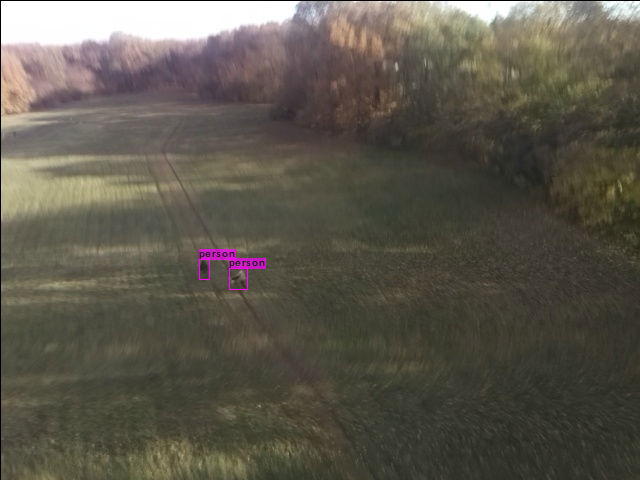
\includegraphics[width=.7\linewidth]{rys03/rozpoznane_yolo.jpg}
	\label{yolo_example}
\end{figure}

\section{Oprogramowanie klienckie}

Aplikacja kliencka pozwala na wykonanie następujących działań:

\begin{itemize}
	\item zaplanowanie przelotu:
	\begin{itemize}
		\item zaplanowanie trasy,
		\item wybór prędkości, z jaką mają być pokonywane konkretne segmenty trasy,
		\item wybór segmentów trasy, podczas których mają być wykonywane zdjęcia,
		\item zaplanowanie godziny wylotu.
	\end{itemize}
	\item podgląd telemetrii w czasie lotu,
	\item przegląd danych teletrycznych zapisanych z poprzednich lotów:
	\begin{itemize}
		\item podlgąd trasy pokonanej przez maszynę,
		\item podgląd wykonanych przez maszynę zdjęć,
				wraz z informacjami o rozpoznanych obiektach,
	\end{itemize} 
\end{itemize}

Najbardziej istotnym z wymagań jest obsługa mapy, która będzie obecna we wszystkich
widokach aplikacji. W systemie została wykorzystana biblioteka \texttt{Leaflet}, 
służąca do wizualizowania danych na mapach. Rysunek \ref{frontend_flight_planner}
zawiera jeden z widoków finalnej wersji aplikacji klienckiej, wykorzystującej
bibliotekę \texttt{leaflet} w komponencie do planowania trasy lotu.
Biblioteka napisana jest z myślą o technologiach  webowych, aplikacja kliencka
została więc zrealizowana jako aplikacja webowa. Wykorzystanym w aplikacji
frameworkiem \texttt{JavaScript} jest~\texttt{VueJS}. 

\begin{figure}[H]
	\centering
	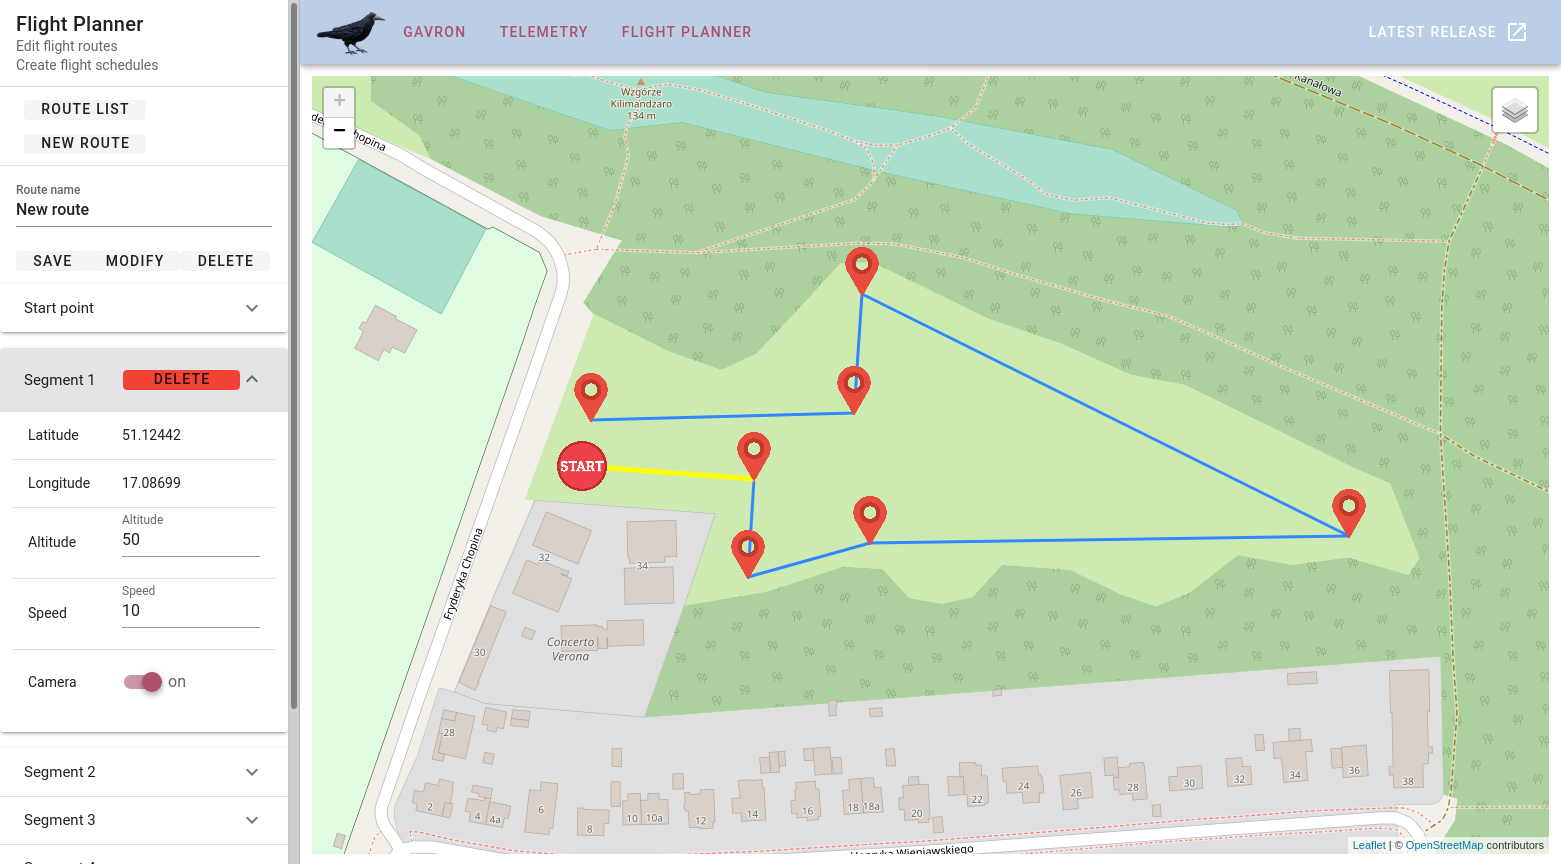
\includegraphics[width=\linewidth]{rys03/flight_planner.png}
	\caption{ Widok aplikacji klienckiej, odpowiedzialny za planowanie tras. }
	\label{frontend_flight_planner}
\end{figure}


\section{Struktura repozytoriów} \label{repo_structure}

\subsection{Konfiguracja \textit{CI/CD}}

Jak zaznaczono w celu pracy (\ref{intro_objective}), system zaopatrzony został w  
mechanizmy automatyzujące testowanie i wdrażanie nowych 
funkcjonalności. Popularne narzędzia do ciągłej integracji, takie jak
\textit{Jenkins}, \textit{Gitlab CI} czy \textit{Travis CI}, wykorzystują specjalny
plik konfiguracyjny umieszczony w repozytorium. Konfiguracja zawiera zestaw kroków,
dzięki którym kod obecny w repozytorium zostanie automatycznie
zbudowany, przetestowany i wdrożony. Wykorzystywanym w projekcie narzędziem \textit{CI/CD}
jest \textit{Gitlab CI}, ktory oczekuje, że w głównym folderze repozytorium będzie 
znajdował się specjalny plik konfiguracyjny, o nazwie \texttt{gitlab-ci.yml}. 
Jest on obecny we wszystkich repozytoriach projektowych.


\subsection{Wspólne punkty stykowe - \texttt{git submodules}}

Komunikacja pomiędzy komponentami systemu realizowana jest za pośrednictwem
pakietów \texttt{Protobuf}, opisanych w rozdziale \ref{protobuf_chapter}.
Każde z repozytoriów musi więc posiadać pliki, zawierające definicje pakietów,
wygenerowane za pomocą kompilatora \texttt{Protobuf}. 

Możliwe jest utrzymywanie kopii definicji pakietów w każdym projektowym repozytorium,
jednak takie rozwiązanie szybko doprowadzi do konieczności wykonywania dużej ilości
ręcznych poprawek w kodzie, za każdym razem gdy zmieni się standard pakietów. 
Nawet przy niewielkiej liczbie repozytoriów, łatwo tu o błąd programisty. 

Napisanie biblioteki z definicjami pakietów nie jest tutaj odpowiednim rozwiązaniem, 
ponieważ biblioteki pisane są zazwyczaj pod konkretny język programowania. Komponenty
systemu, które przetwarzają telemetrię są napisane w językach \textit{Python} i 
\textit{TypeScript} -- nie jest więc możliwe napisanie dla nich wspólnej biblioteki.

System kontroli wersji \texttt{git} zawiera funkcjonalność
\texttt{git submodules}\cite{git_submodules}, która została wykorzystana
w projekcie do rozwiązania problemu wspólnych definicji pakietów.

Definicje pakietów, wraz z wygenerowanymi implementacjami w wielu językach, utrzymywane 
są w osobnym repozytorium, które pobierane jest jako submoduł dla pozostałych projektów.
Dzięki temu, możliwa jest aktualizacja repozytorium z definicjami pakietów, a następnie
pobranie nowych definicji do wszystkich innych  repozytoriów, które wykorzystują
submoduł z definicjami. 


\newpage
\section{Architektura systemu - podsumowanie}

Rysunek \ref{technologies_diagram} opisuje wykorzystywane w projekcie
technologie i sprzęt.

\begin{figure}[H]
\centering\small

\hspace{-1.2cm}
\begin{forest}
	% forest preamble: determine layout and format of tree
	direction switch, 
	for tree={fork sep=2em, l sep=0.5cm, s sep=0.6cm}
	[ System inspekcji obszarów ,yshift=3em,alias=LP, s sep=2.2cm
	  [ \textbf{Dron}
		[ Kontroler lotu 
		  [ \texttt{ArduPilot} ]
		]
		[ Komputer pokładowy, name=flight_computer
		 [ Raspberry Pi ]
		 [ \texttt{Dronekit-Python} ]
		 [ \texttt{pymavlink} ]
		]
	  ]
	  [ \textbf{Serwer webowy}, %yshift=0.5cm
		[ Serwer telemetrii, name=telem_server
			[ \texttt{asyncio } ]
			[ \texttt{UDP} ]
			[ \texttt{WebSocket} ]
		]
		[ Rest API: odczyt i zapis
		  [ \texttt{django} ]
		]
		[ Przesył zdjęć 
		  [ \texttt{imagezmq} ]
		]
		[ Sztuczna inteligencja
		  [ \texttt{yolo} ]
		]
	  ]
	  [ \textbf{Aplikacja kliencka}, xshift=0.1cm
		[ \texttt{VueJS} 
			[ \texttt{Leaflet} ]
			[ \texttt{WebSocket}, name=front_websocket]
		]
	  ]
	]
	\node
		[entity, yshift=-17cm, xshift=4.5cm, align=center](definitions)
		{ Definicje wiadomości \texttt{protobuf} };
	\draw[->] (definitions) to[out=north east, in=south east] node[fill=white,pos=.6]{Submoduł} (telem_server); % leave fill=white away in order to get your image. pos=. is optional. Default would be .5
	\draw[->] (definitions) to[out=north east, in=south east] node[fill=white,pos=.6]{Submoduł} (front_websocket); % leave fill=white away in order to get your image. pos=. is optional. Default would be .5
	\draw[->] (definitions) to[out=west, in=south east] node[fill=white,pos=.6]{Submoduł} (flight_computer); % leave fill=white away in order to get your image. pos=. is optional. Default would be .5
\end{forest}
\caption{
	Architektura systemu - wykorzystane technologie
}
\label{technologies_diagram}
\end{figure}


\chapter{Podsumowanie}

\section{Wyniki testów}
\section{Osiągnięta sprawność}
\section{Pola do poprawy}
\section{Wnioski}

%%%2. środowisko do pisania kodu latexa: 
%%%( )
%%%3. viewer pdf-ów, pozwalający na nawigację zwrotną: Sumatra PDF 3.0
%%%(http://www.sumatrapdfreader.org/download-free-pdf-viewer.html)
%%%
%%%- o konfiguracji texniccenter do współdziałania z sumatra pdf można poczytać sobie na stronie:
%%%http://tex.stackexchange.com/questions/116981/how-to-configure-texniccenter-2-0-with-sumatra-2013-2014-2015-version
%%%(można znaleźć też inne tutoriale)
%%%
%%%4. środowisko do zarządzania bibliografią: JabRef
%%%(http://jabref.sourceforge.net/download.php)
%%%
%%%Polecam też instalację pod windowsami następujących narzędzi:
%%%- Sumatra PDF - przeglądarka pdf umożliwiająca nawigację pomiędzy
%%%edytowanym tekstem a przeglądanym dokumentem (podglądanie tekstu w
%%%TeXnicCenter umieszcza kursor w odpowiednim miejscu w pdfie, podwójne
%%%kliknięcie w pdfie ustawia kursor w edytorze tekstu).
%%%- JabRef - narzędzie do przygotowywania bibliografii.
%%%
%%%
%%%Uwaga: tytuł powinien zmieścić się w okienku kolorowej okładki (którą
%%%powinna dostarczyć uczelniana administracja). Proszę posterować
%%%parametrami, aby "wpasować" w okienko własny tekst.
%%%
%%%Do ASAPa należy wprowadzić pracę dyplomową/projekt inżynierski w pliku o nazwie:
%%%
%%%W04_[nr albumu]_[rok kalendarzowy]_[rodzaj pracy] (szczegółowa instrukcja pod adresem asap.pwr.edu.pl)
%%%
           %%%Przykładowo:
        %%%­W04_123456_2015_praca inżynierska.pdf     - praca dyplomowa inżynierska
        %%%W04_123456_2015_projekt inżynierski.pdf   - projekt inżynierski
        %%%W04_123456_2015_praca magisterska.pdf  - praca dyplomowa magisterska
%%%
              %%%rok kalendarzowy ? rok realizacji kursu „Praca dyplomowa” (nie rok obrony) 

% \chapter{Wdrażanie systemu} \label{chapter_deployment}

% Napisać jeszcze raz, wtf
Jak zaznaczono~w zakresie pracy (\ref{intro_objective}),
architektura systemu ma pozwalać na automatyzację wdrożeń.
W niniejszym rozdziale opisane są technologie~i praktyki, które zostały 
zastosowane, aby zautomatyzować wdrażanie systemu.

\section{Konteneryzacja}

Wszystkie elementy systemu (za wyjątkiem oprogramowania na dronie) są uruchamiane~w kontenerach.
Wykorzystanym systemem konteneryzacji jest \texttt{docker}\cite{docker}.
Konteneryzacja pozwala na zupełne zautomatyzowanie
procesu budowania oprogramowania~i instalacji koniecznych
składników środowiska uruchomieniowego. Aby zbudować kontener zawierający
aplikację, programista musi napisać skrypt,~w wyniku
którego~w kontenerze zostanie zainstalowane konieczne 
do uruchomienia aplikacji oprogramowanie. Proces instalacji~i konfiguracji
wymaganych bibliotek jest więc automatyczny~i deterministyczny -- wszystko
zależy tylko~i wyłącznie od skryptu budującego kontener.

Konteneryzacja ułatwia proces przenoszenia oprogramowania~z maszyny na maszynę. Raz zbudowany
kontener może zostać uruchomiony na dowolnej nowej maszynie, bez konieczności instalowania 
czy konfigurowania bibliotek czy programów. 

\subsection{Zachowywanie stanu systemu plików~w kontenerze} \label{volumes}

Ważną różnicą, jaka odróżnia kontenery od aplikacji zainstalowanych~w sposób konwencjonalny, jest \textbf{bezstanowość}. Jeśli komputer,
na którym działają kontenery zostanie zresetowany, bądź kontener zostanie
usunięty~i utworzony na nowo (na przykład~w celu aktualizacji), system
plików~w kontenerze zostanie zresetowany do stanu,~w jakim znajdował się ~w momencie uruchomienia (takim, jaki jest zapisany~w \textit{obrazie kontenera}).

\texttt{Docker} pozwala rozwiązać ten problem za pomocą mechanizmu 
woluminów (\textit{docker volumes})\cite{docker_volumes}.
Za pomocą woluminów, dowolny fragment systemu
plików kontenera może zostać zmapowany do nieulotnej pamięci komputera, na którym 
działa kontener.~W ten sposób zapewnia się persystencję baz danych lub innych
plików, które mają być przechowywane przez aplikację.\\ % newline CAN be removed

\textit{Uwaga:} nie wszystkie kontenery potrzebują zachowywać pliki -- kontener
odpowiedzialny za hostowanie statycznej strony internetowej nie potrzebuje
zapamiętywać zmian, ponieważ pliki strony nie zmieniają się podczas hostowania. 

\section{Automatyczne budowanie~i testowanie komponentów systemu}

Jak wspomniano~w rozdziale \ref{repo_structure}, poświęconym strukturze repozytoriów,
wszystkie repozytoria zawierają plik \texttt{.gitlab-ci.yml}. Plik ten definiuje skrypty,
jakie wykona potok \texttt{CI/CD}, gdy do repozytorium zostanie dodany nowy kod.
Diagram ilustrujący proces pracy programisty~z potokiem \textit{CI/CD} zawarty jest
na rysunku \ref{ci_workflow}.

\begin{figure}[H]
	\centering\small

\tikzstyle{arrow} = [thick,->,>=stealth]
\begin{tikzpicture}[node distance=4cm,auto,>=stealth']
    
    \node[] (programmer) {Programista};
    \node[right of = programmer] (repo) {Repozytorium};
    \node[right of = repo] (ci_cd) {Potok \texttt{CI/CD}};
    \node[right of = ci_cd] (registry) {Rejestr kontenerów};

    \node[below of = programmer, node distance=6cm] (programmer_ground) {};
    \node[below of = repo, node distance=6cm] (repo_ground) {};
    \node[below of = ci_cd, node distance=6cm] (ci_cd_ground) {};
    \node[below of = registry, node distance=6cm] (registry_ground) {};
    %
    \draw (repo) -- (repo_ground);
    \draw (programmer) -- (programmer_ground);
    \draw (ci_cd) -- (ci_cd_ground);
    \draw (registry) -- (registry_ground);


    \draw[->] ($(programmer)!0.20!(programmer_ground)$) -- node[above,scale=1,midway]{Nowy \textit{commit}} ($(repo)!0.20!(repo_ground)$);
    % \draw[<-] ($(programmer)!0.35!(programmer_ground)$) -- node[above,scale=1,midway]{Text} ($(repo)!0.35!(repo_ground)$);
    \draw[->,align=center] ($(repo)!0.35!(repo_ground)$) -- node[above,scale=1,midway]{Zainicjowanie procesu\\budowania} ($(ci_cd)!0.35!(ci_cd_ground)$);

    \draw[->,align=center] ($(ci_cd)!0.60!(ci_cd_ground)$) -- node[above,scale=1,midway]{ Wysłanie zbudowanego \\~i przetestowanego \\ konteneru do rejestru} ($(registry)!0.60!(registry_ground)$);
    
    \draw[<-,align=center] ($(repo)!0.70!(repo_ground)$) -- node[above,scale=1,midway]{Status~i logi \\z potoku \texttt{CI/CD}} ($(ci_cd)!0.70!(ci_cd_ground)$);
    \draw[<-,align=center] ($(programmer)!0.90!(programmer_ground)$) -- node[above,scale=1,midway]{Informacja, czy \\ \textit{commit} przeszedł testy} ($(repo)!0.90!(repo_ground)$);
\end{tikzpicture}
	\caption{
      Diagram sekwencji, opisujący proces automatycznej budowy i testowania kontenerów 
	}
	\label{ci_workflow}
\end{figure}

Ponieważ konteneryzacja pozwala na zupełne zautomatyzowanie procesu budowania,
skrypty~w potoku \texttt{CI/CD} są~w stanie samodzielnie zbudować kontener,
zawierający konkretny komponent systemu. Następnie, kontener poddawany jest testom
(opisanym~w rozdziale \ref{chapter_tests}). Po przejściu testów, kontener wysyłany jest
do \textit{rejestru kontenerów} -- specjalnego repozytorium, w~którym można
przechowywać~i wersjonować kontenery. Skrypt potoku \texttt{CI/CD} automatycznie oznacza
kontener za pomocą nazwy brancha, na której został zbudowany. Kontenery pochodzące~z brancha
\textit{master}, uruchamiane są na serwerze produkcyjnym. Przykładowa konfiguracja
\textit{Gitlab CI}, wykorzystywana~w repozytorium aplikacji klienckiej opisana została~w listingu
\ref{list:ci_cd_frontend}.

\begin{lstlisting}[language=yml, label=list:ci_cd_frontend,caption={Plik konfiguracyjny \textit{Gitlab CI}, budujący aplikację kliencką }, basicstyle=\footnotesize\ttfamily]
# Definicje zmiennych, wpływających na proces budowania
variables:
  # Wywołuje automatyczne pobranie submodułów,
  # przed przystąpieniem do budowania 
  GIT_SUBMODULE_STRATEGY: recursive
 
  # Zapewnia dostęp do dockera z poziomu systemu CI/CD
  DOCKER_HOST: tcp://docker:2375
  DOCKER_TLS_CERTDIR: "" 

  # Specyfikuje nazwę kontenera, który zostanie zbudowany 
  IMAGE_NAME: "registry.gitlab.com/academic-aviation-club/gavron/frontend"

# Przed wykonaniem danego skryptu budującego, wykonywane jest logowanie
# do rejestru dockera - umożliwi to zapisanie w nim 
# zbudowanego obrazu aplikacji. Zmienna $GITLAB_DEPLOY_TOKEN
# przypisywana jest w ustawieniach repozytorium
before_script:
  - docker login -u baczek-vps -p $GITLAB_DEPLOY_TOKEN registry.gitlab.com

# Zawsze budowany jest obraz testowy, który zostanie
# później wykorzystany do testów systemowych 
build_testing_image:
  stage: build
  # Zapewnia dostęp do dockera w ramach zadania `build_testing_image`
  services:
    - docker:19.03.12-dind
  image: docker:19.03.12
  
  # Skrypt wpierw buduje obraz dockera, zawierający aplikację.
  # Następnie uruchamia na obrazie testy jednostkowe. Jeśli testy
  # nie zwrócą błędu, obraz jest wysyłany do rejestru.
  # Na obrazach w rejestrze wykonywane są testy systemowe.
  script:
  - docker build -f docker/test.dockerfile -t $IMAGE_NAME:test_$CI_COMMIT_REF_NAME .
  - docker run $IMAGE_NAME:$CI_COMMIT_REF_NAME "npm run test"
  - docker push $IMAGE_NAME:test_$CI_COMMIT_REF_NAME

# Tylko dla brancha `master`, budowany jest obraz 
# produkcyjny, który zostanie uruchomiony na serwerze
build_prod_image:
  stage: build
  services:
	- docker:19.03.12-dind	
  # `only` pozwala na wybranie brancha, na którym działa dany skrypt
  only:
    - master
  image: docker:19.03.12
   
  script:
  - docker build -f docker/Dockerfile -t $IMAGE_NAME:$CI_COMMIT_REF_NAME .
  - docker run $IMAGE_NAME:$CI_COMMIT_REF_NAME "npm run test"
  - docker push $IMAGE_NAME:$CI_COMMIT_REF_NAME
\end{lstlisting}

Wszystkie logi, jakie potok CI/CD zbierze~w trakcie budowania~i testowania obrazu~z aplikacją są
dostępne dla programisty -- pozwala to odnaleźć błędy, które pojawiły się~w procesie budowania oraz
sprawdzić wyniki testów. Systemy obsługi repozytorium (taki jak \textit{GitHub}, \textit{BitBucket}
czy \textit{GitLab}), wyświetlają informacje~o tym, czy dany commit przeszedł testy~w potoku 
\textit{CI/CD}, ułatwiając odnajdywanie commitów zawierających błędy. Przykład tej funkcji
zilustrowany jest na rysunku \ref{gitlab_ci_history}.

\begin{figure}[H]
  \centering
  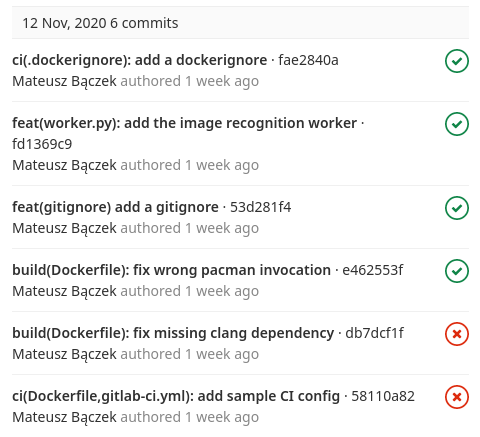
\includegraphics[width=.7\linewidth]{rys04/gitlab_ci_commit_status.png}
  \caption{ Historia zmian~w kodzie~w serwisie \textit{GitLab}.
  Ikony po prawej stronie informują, czy dany commit przeszedł testy~w potoku CI/CD }
	\label{gitlab_ci_history}
\end{figure}

\section{Automatyczne aktualizacje kontenerów} \label{ouroboros}

Pobranie~i uruchomienie kontenera, zawierającego dany komponent systemu
nie wymaga przechodzenia przez proces instalacji czy konfiguracji -- wystarczy
pobrać obraz kontenera~z rejestru~i uruchomić go:

\begin{lstlisting}[language=bash, label=list:docker_clone_run_example,caption={Pobranie~i uruchomienie obrazu dockera, zawierającego aplikację}, basicstyle=\footnotesize\ttfamily]
# Zapisane jako zmienna, aby poprawić czytelność przykładu 
IMAGE=registry.gitlab.com/academic-aviation-club/gavron/frontend:master

docker pull $IMAGE
docker run \
    -d \ # detach: kontener działa w tle, nie wysyła logów do terminala
    -p 5000:5000 \ # mapuje port 5000 z kontenera do portu na komputerze  
    --name frontend \ # Nadaje nazwę uruchomionemu kontenerowi
    $IMAGE # Nazwa obrazu do uruchomienia 
\end{lstlisting}
~W przypadku, gdy na serwerze działa już kontener~z aplikacją, należy
pobrać nowy obraz kontenera, usunąc obecnie działający kontener~i uruchomić
nowy obraz:

\begin{lstlisting}[language=bash, label=list:docker_update_container,caption={Aktualizacja kontenerów}, basicstyle=\footnotesize\ttfamily]
IMAGE=registry.gitlab.com/academic-aviation-club/gavron/frontend:master

docker pull $IMAGE # Pobranie najnowszej wersji kontenera

# Nazwa kontenera nadana w poprzednim przykładzie, za pomocą --name
docker stop frontend

# Usunięcie kontenera w starej wersji (jego stanu, zmian w systemie plików)
docker rm frontend

# Tak samo jak w przykładzie powyżej
docker run \
    -d \ # detach: kontener działa w tle, nie wysyła logów do terminala
    -p 5000:5000 \ # mapuje port 5000 z kontenera do portu na komputerze  
    --name frontend \ # Nadaje nazwę uruchomionemu kontenerowi
    $CONTAINER # Nazwa kontenera do uruchomienia 
\end{lstlisting}
~W przypadku wielu równolegle działających kontenerów, ręczna aktualizacja 
każdej działającej aplikacji jest zadaniem niepotrzebnie czasochłonnym.
Wprowadza też dodatkowy punkt,~w którym może zajść pomyłka -- na przykład
pominięcie jednego~z kontenerów przy aktualizacji.

Projekt wykorzystuje narzędzie \texttt{Ouroboros} do automatycznej aktualizacji
uruchomionych na serwerze kontenerów. \texttt{Ouroboros}~w regularnych odstępach
czasu sprawdza, czy uruchomione na serwerze kontenery nie wymagają aktualizacji.
Jeśli~w rejestrze dostępna jest nowa wersja obrazu kontenera, pobiera ją~i zastępuje
nią obecnie działający kontener.

Dzięki zastosowaniu narzędzia \texttt{Ouroboros}, w trakcie testów w terenie 
udało się znacznie usprawnić aktualizacje infrastruktury systemu. W przypadku
pojawienia się błędu, programiści musieli jedynie zaktualizować kod w repozytorium --
potok \textit{CI/CD} automatycznie budował poprawioną wersję kontenera, \texttt{Ouroboros}
aktualizował serwer produkcyjny. Po dodaniu nowego kodu do repozytorium, uaktualniona
wersja aplikacji pojawiała się na serwerze po mniej niż pięciu minutach.

\section{Orkiestracja systemu złożonego~z wielu kontenerów -- \texttt{docker-compose}}

Finalnie, infrastruktura internetowa systemu składa się~z sześciu
jednocześnie działających kontenerów dockerowych:

\begin{enumerate}
  \item Kontener serwujący stronę internetową~z aplikacją kliencką,
  \item Kontener~z serwerem API,
  \item Kontener~z serwerem \texttt{imagezmq},
  \item Kontener~z systemem telemetrii,
  \item Kontener~z programem \texttt{ouroboros} (opisanym~w rozdziale \ref{ouroboros}),
  \item Kontener~z systemem do rozpoznawania obrazów. 
\end{enumerate}

\noindent
Każdy kontener musi zostać odpowiednio skonfigurowany~w momencie uruchamiania.
Konfiguracja poszczególnego kontenera obejmuje:

\begin{itemize}
  \item Przypisanie limitów zasobów (n.p. maksymalny procent wykorzystania procesora)
  \item Udostępnienie portów serwera, które może wykorzystywać dany kontener,
  \item Przypisanie woluminów systemu plików serwera,~w celu zapewnienia persystencji
        danych, zapisywanych przez kontener (opisane~w rozdziale \ref{volumes}),
  \item Zdefiniowanie reguł automatycznego restartu kontenera (na przykład gdyby proces
        działający~w kontenerze uległ awarii),
  \item Określenie zmiennych środowiskowych, które mogą wpływać na zachowanie się
        procesów wewnątrz kontenera (przykładowo, kontener \texttt{ouroboros} pozwala
        za pomocą zmiennych środowiskowych określić, jak często mają być sprawdzane
        aktualizacje kontenerów).
\end{itemize}

Narzędzie \texttt{docker-compose} pozwala zebrać całą konfigurację kontenerów do 
jednego pliku konfiguracyjnego \cite{docker_compose}.~W ten sposób, po uzyskaniu
dostępu do rejestru~z kontenerami, zawierającymi komponenty systemu, możliwe jest
natychmiastowe pobranie~i uruchomienie systemu~z właściwą konfiguracją kontenerów.


% \chapter{Testy systemu} \label{chapter_tests}

Jak zaznaczono w celu pracy (\ref{intro_objective}), prototyp systemu
ma być w pełni testowalny. Testy wykonywane są wewnątrz systemu ciągłej integracji 
(\textit{CI/CD}), opisanym w rozdziale \ref{chapter_deployment}. Poniższy rozdział opisuje
rozwiązania zastosowane w celu przetestowania działania systemu,
zanim został on uruchomiony na prawdziwym dronie.

\section{Testy jednostkowe}

Komponenty systemu zaopatrzone są w testy jednostkowe, co pozwala na
sprawdzenie działania kodu w zakresie poszczególnego komponentu.
Przykład testu jednostkowego wykorzystywanego w systemie
zawarty jest w listingu \ref{list:unit_test_example}.

\begin{lstlisting}[
    language=Python,
    label=list:unit_test_example,
    caption={
        Test jednostkowy modułu sterującego uruchamianiem symulatoru drona.
        test sprawdza, czy symulator uruchamia się, oraz czy zostaje poprawnie
        zamknięty po wywołaniu metody \texttt{.stop()}.
    },
    basicstyle=\footnotesize\ttfamily
]
def test_container_lifecycle():
	# Check how many docker containers are running
	num_of_containers = int(check_output('docker ps | wc -l', shell=True))

	print('setting up the runnner')
	runner = SitlDockerHelper('ArduCopter', run_in_background=True)

	print('running the container')
	runner.run()
	sleep(10)

	new_num_of_containers = int(
        check_output('docker ps | wc -l', shell=True)
    )

	# Check if the number of running containers has increased
	assert num_of_containers + 1 == new_num_of_containers

	print('stopping')
	runner.stop()

	# Check if the num of running containers is back to the start state
	assert int(check_output('docker ps | wc -l', shell=True)) == num_of_containers
\end{lstlisting}

Wykonywanie testów w systemie \textit{CI/CD} zwiększa sprawność
pracy z systemami kontroli wersji. W przypadku implementowania nowej 
funkcji na gałęzi (\textit{branch}), system \textit{CI/CD} pozwala określić,
czy nowa funkcjonalność nie destabilizuje systemu -- ostrzegając przed 
przyjęciem na główną gałąź (\textit{master branch}) kodu, który nie przeszedł
testów jednostkowych. Rysunek \ref{failed_pipeline} przedstawia przykład
takiego zachowania w usłudze \textit{GitLab}.

\begin{figure}[H]
	\centering
	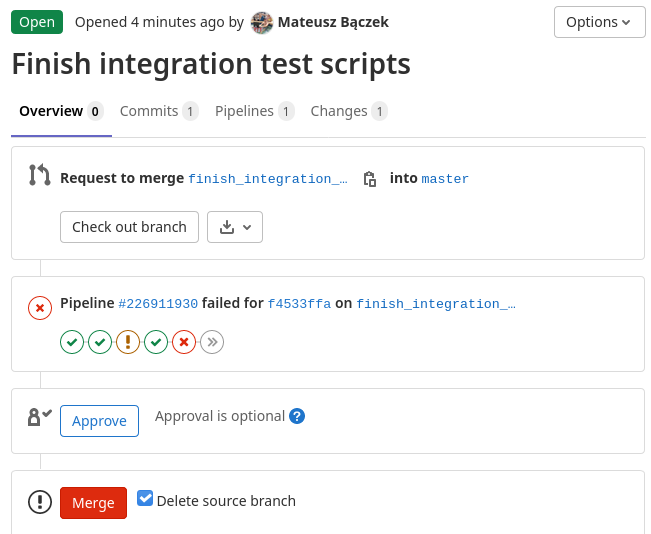
\includegraphics[width=0.8\linewidth]{rys05/failed_pipeline.png}
    \caption{
        Widok interfejsu scalania gałęzi w serwisie \textit{GitLab}.
        Gałąź \texttt{finish\_integration\_tests} nie przechodzi testów
        w systemie \textit{CI/CD}. Administrator repozytorium natychmiast
        otrzymuje informację, że kod nie jest jeszcze gotowy do scalenia.
    }
	\label{failed_pipeline}
\end{figure}


\section{Testy integracyjne}

Realizowany w pracy system nie ogranicza się do pojedynczego,
samodzielnego komponentu, zawiera kilka równolegle działających
usług. testy jednostkowe nie są w takim przypadku wystarczające,
aby gruntownie sprawdzić poprawność działania kodu. 

Dodatkowym wyzwaniem przy projektowaniu testów jest interakcja z dronem,
którego kontroler lotu komunikuje się z systemem za pośrednictwem 
interfejsu \texttt{UART}, podłączonego do komputera pokładowego.
Błąd w komunikacji z kontrolerem lotu może doprowadzić do 
rozbicia maszyny, straty są tutaj zupełnie realne, inaczej
niż w przypadku testowania systemów pracujących jedynie na serwerach. 

\subsection{
    Symulacja i symulatory
    \color{white}\cite{simulation_and_simulacra}}

Symulatory lotu są szeroko wykorzystywane w przemyśle lotniczym
\cite{simulation_and_simulators}. Amatorskie otwartoźródłowe kontrolery
lotu nie są tutaj wyjątkiem -- jak wspomniano~w rozdziale poświęconym
kontrolerom lotu (\ref{flight_controller}), wykorzystywane w projekcie 
oprogramowanie \textit{ArduPilot} ma możliwość pracy w trybie \textit{SITL}
(\textit{software in the loop}). Jest to możliwe dzięki specjalnym opcjom,
które można ustawić w trakcie kompilacji. Opcje umożliwiają przemapowanie
interfejsów kontrolujących peryferia samolotu na ich wirtualne odpowiedniki,
które podłączane są do symulatora. Kod sterujący zachowaniem drona 
oraz dane telemetryczne pozostają takie same jak w przypadku
pracy na prawdziwej maszynie. Szczegółowy diagram 
ilustrujący przemapowywane peryferia kontrolera lotu 
zawarty jest na rysunku~\ref{sitl_diagram}.

\begin{figure}[H]
	\centering
	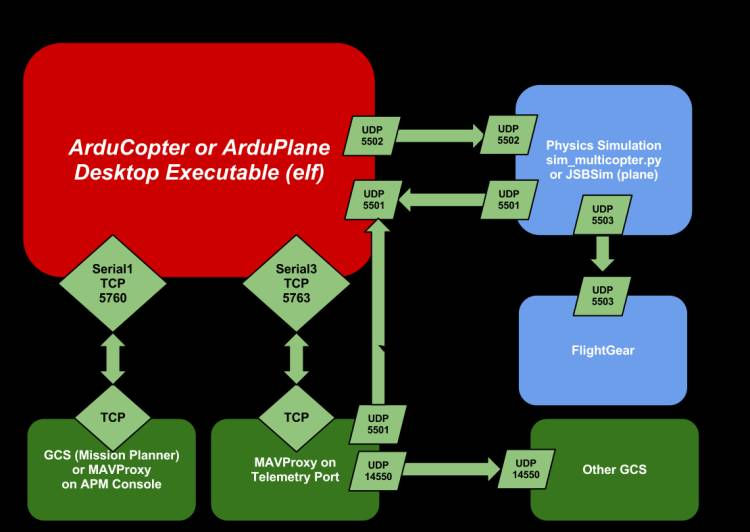
\includegraphics[width=0.9\linewidth]{rys05/sitl.jpg}
    \caption{
        Diagram zaczerpięty z dokumentacji \textit{ArduPilota}
        \cite{ardupilot_sitl}, ilustrujący działanie symulatora SITL.
    }
	\label{sitl_diagram}
\end{figure}


Ponieważ jedyna zmiana w wynikowym pliku wykonywalnym
z kontrolerem lotu to przemapowane interfejsy peryferiów,
komunikacja z kontrolerem lotu nadal działa w dokładnie
taki sam sposób. Kod, który był w stanie skomunikować
się z kontrolerem lotu działającym w trybie \textit{SITL},
będzie na pewno działał również na prawdziwej maszynie
(wyjątkiem byłaby oczywiście usterka sprzętowa, jednak takie
problemy leżą poza zakresem odpowiedzialności kodu).

Listing \ref{list:connecting_to_ardupilot_or_sitl} ilustruje,
jak zależnie od parametru konfiguracyjnego, skrypt sterujący 
dronem będzie próbował podłączyć się do prawdziwej maszyny lub
do symulatora. Jedyną różnicą są parametry w konstruktorze
obiektu połączenia, pozostały kod nie musi być modyfikowany
gdy przechodzi się z symulatora na prawdziwego drona.

\begin{lstlisting}[
    language=Python,
    label=list:connecting_to_ardupilot_or_sitl,
    caption={
        Przykład kodu łączącego się z prawdziwym dronem lub 
        z symulatorem lotu, zależnie od wartości parametru
        \texttt{USE\_SITL}. Utworzony obiekt \texttt{connection},
        reprezentujący połączenie, zawsze zachowuje się w taki
        sam sposób, niezależnie czy wykorzystywana jest
        prawdziwa maszyna czy symulator. 
    },
    basicstyle=\footnotesize\ttfamily
]
if USE_SITL:
    connection = mavutil.mavlink_connection(
        'udpin:0.0.0.0:14551' # Połączenie z symulatorem na porcie UDP
    )

else:    
    connection = mavutil.mavlink_connection(
        '/dev/ttyS0', # Połączenie z dronem za pomocą interfejsu UART
        baud=57600
    )
# Dalszy kod wykorzystujący obiekt `connection`.
# Nie ma znaczenia czy `connection` oznacza połączenie
# do symulatora czy do prawdziwego drona/samolotu
\end{lstlisting}

\subsection{\textit{SITL} i automatyczne testy w systemie \textit{CI/CD}}

Jak opisano w rozdziale \ref{chapter_deployment}, wszystkie komponenty systemu
docelowo uruchamiane są w kontenerach. Takie rozwiązanie pozwala na zagwarantowanie
poprawnego wdrożenia systemu na serwerze produkcyjnym. Równocześnie, kontenery wysyłane
na serwer produkcyjny można wcześniej przetestować w wirtualnym środowisku testowym.

Na potrzeby projektu, symulator kontrolera lotu został zkonteneryzowany i wykorzystany
w \textit{CI/CD} do testów integracyjnych, angażujących wszystkie komponenty systemu.
Zespół pracujący nad projektem używał gotowego kontenera z symulatorem,
aby przeprowadzać testy na własnych maszynach. Takie rozwiązanie eliminuje wszystkie
problemy, jakie mogą pojawić się podczas wykorzystywania oprogramowania którego
konfiguracja jest bardzo złożona -- tak jak w przypadku symulatora lotu.

\subsection{Budowanie testów integracyjnych z wykorzystaniem \textit{Gitlab CI}}

Do uruchamiania testów integracyjnych przeznaczony został dedytkowany serwer
Linux. Serwer służył za platformę, na której uruchamiane były wszystkie 
komponenty systemu. Diagram \ref{integration_tests_diagram} ilustruje 
sposób wykorzystywania dedykowanego serwera w celu przeprowadzenia 
testów integracyjnych.

\begin{figure}[H]
	\centering
	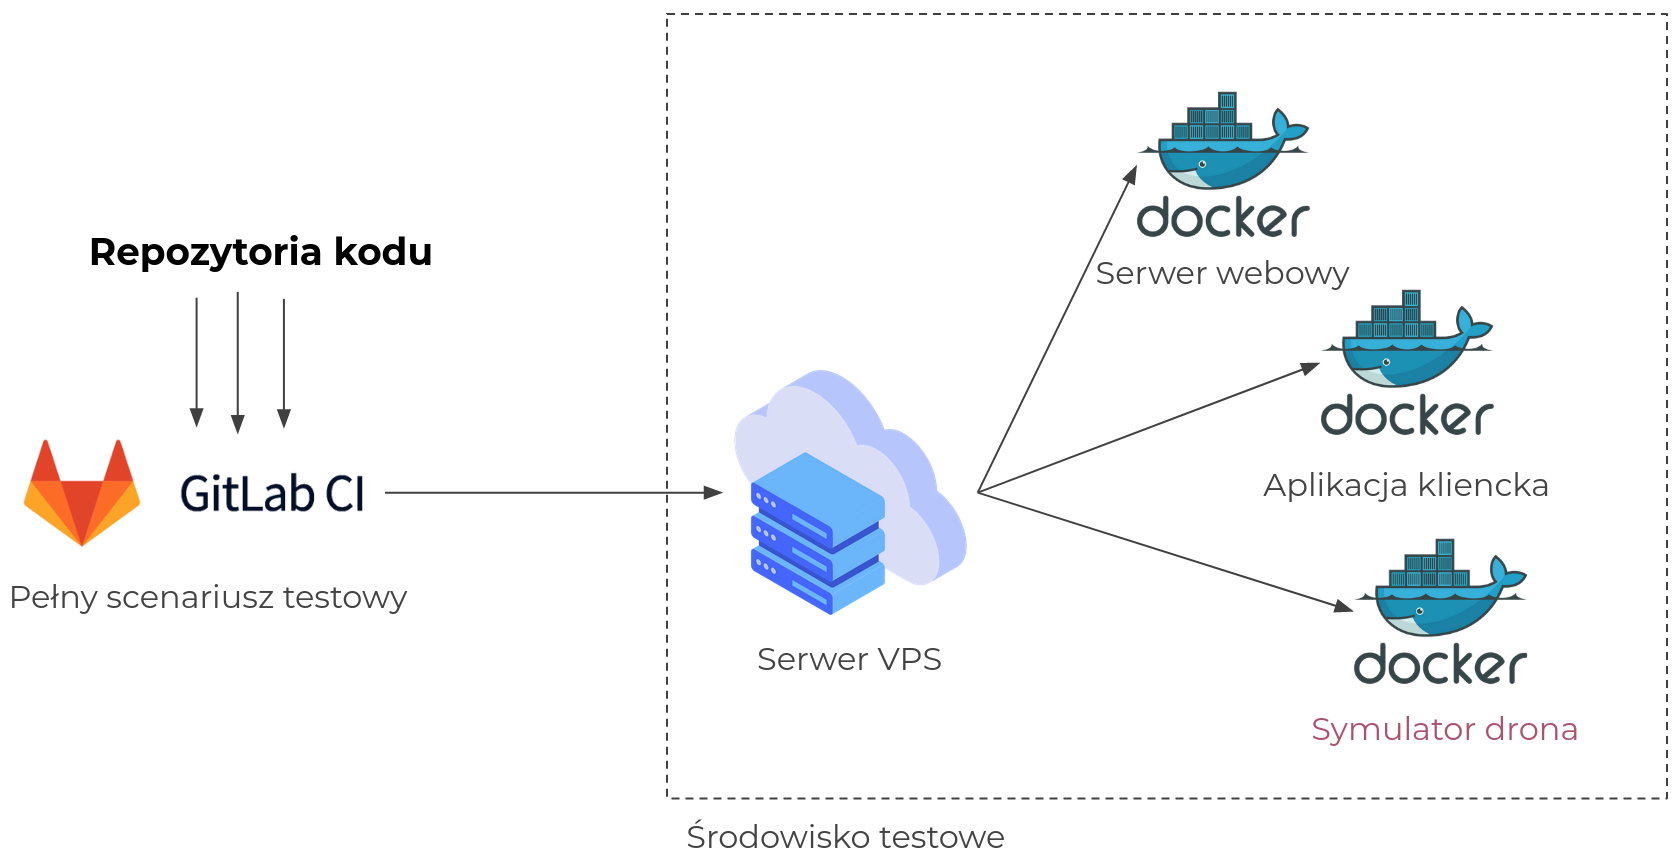
\includegraphics[width=\linewidth]{rys05/integration_tests_diagram.png}
    \caption{
        Pełne testy integracyjne na dedykowanym serwerze.
    }
	\label{integration_tests_diagram}
\end{figure}

\subsection{Konfiguracja serwera zarządzanego przez \textit{Gitlab CI}}

Platforma \textit{GitLab} umożliwia uruchamianie testów na własnej
infrastrukturze, w ramach usług dostępnych dla darmowych kont.
Infrastruktura platformy domyślnie pozwala jedynie
na testowanie wewnątrz izolowanych kontenerów \texttt{docker}.
Jest to rozwiązanie zupełnie wystarczające w przypadku testów jednostkowych.
Uruchomienie pełnego systemu w sztucznym środowisku wymaga jednak
większej kontroli nad serwerem testowym. \textit{Gitlab CI} pozwala
na podłączenie własnych serwerów do swojej sieci -- dzięki takiemu rozwiązaniu
użytkownicy mogą wykorzystywać pełne możliwości systemu ciągłej integracji.

Podłączony do systemu serwer wykonuje skrypty uruchamiające testy integracyjne
wprost na serwerze, co pozwala na równoległe uruchomienie wielu kontenerów 
\texttt{docker} oraz monitorowanie ich pracy z zewnątrz -- jak pokazano
na diagramie \ref{integration_tests_diagram}.

\subsection{Definiowanie wieloetapowych testów integracyjnych}

W ramach testów integracyjnych testowane są wpierw pojedyncze kontenery --
nie są to jednak testy jednostkowe. Uruchamiany jest cały kontener zawierający
komponent systemu, następnie jest on testowany przez zewnętrzny skrypt.
W przypadku aplikacji klienckiej, uruchamiana jest sterowana automatycznie 
przeglądarka internetowa, która symuluje zachowanie prawdziwego użytkownika,
tworząc nową trasę przelotu drona. W przypadku serwera \textit{REST API}, wykonywane
są zapytania \textit{http} weryfikujące poprawność działania \textit{API}.

Po przetestowaniu pojedynych kontenerów, uruchamiane są testy angażujące
wiele kontenerów -- sprawdzające czy komponenty systemu będą ze sobą współpracowały.
Przykładowy scenariusz testowy zawiera:

\begin{enumerate}
    \item Uruchomienie kontenerów:
    \begin{itemize}
        \item symulatora kontrolera lotu,
        \item aplikacji sterującej dronem,
        \item aplikacji klienckiej
        \item serwera telemetrii
        \item serwera API.
    \end{itemize}
    \item Wykorzystanie zdalnie sterowanej przeglądarki w
            celu dodania nowej trasy przelotu w aplikacji klienckiej.
    \item Sprawdzenie, czy w aplikacji klienckiej pojawi się telemetria z drona,
            wykonującego zaplanowaną trasę.
\end{enumerate}

Taki test angażuje wszystkie uruchamiane komponenty. Skrypt wykonujący test
musi jedynie sterować aplikacją kliencką i weryfikować, czy pojawiają się
w niej dane pochodzące z pozostałych komponentów systemu.

\subsubsection{Etapy testów w \textit{GitLab CI}}

Platforma \textit{GitLab CI} pozwala na podzielenie testów na etapy. 
Każdy etap składa się z określonej liczby zadań. Aby system \textit{CI/CD}
mógł przejść do kolejnego etapu, muszą zostać wykonane wszystkie zadania 
z poprzednich etapów. W przypadku testów integracyjnych oznacza to, że wpierw
zweryfikowane musi zostać działanie wszystkich kontenerów składających się
na system, następnie testowane są interakcje między komponentami. 
Finalny zestaw testów integracyjnych (\textit{test pipeline}), które były
wykonywane na systemie ilustruje rysunek \ref{pipeline_gitlab_ci}.

\begin{figure}[H]
	\centering
	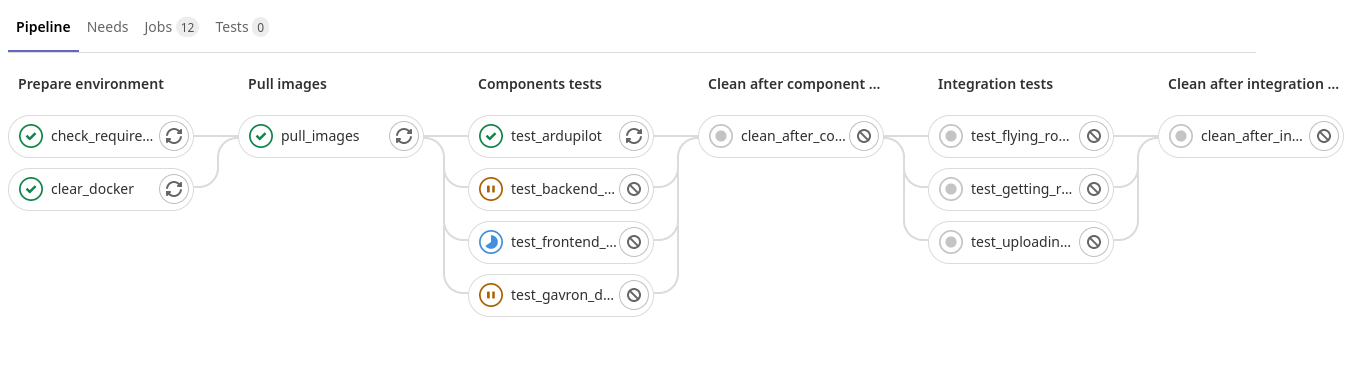
\includegraphics[width=\linewidth]{rys05/pipeline.png}
    \caption{
        Interfejs \textit{GitLab CI} prezentujący postęp w wykonywaniu
        wieloetapowych testów integracyjnych.
    }
	\label{pipeline_gitlab_ci}
\end{figure}

\section{Testy w terenie}


% \chapter{Podsumowanie}


W trakcie testów w terenie wszystkie komponenty systemu bezkonfliktowo współgrały
ze sobą. Jest to zasługa faktu, że były wcześniej regularnie sprawdzane
wewnątrz środowiska testowego. Z punktu widzenia infrastruktury sieciowej,
testy w terenie nie różniły się niczym od testów wykonywanych na symulatorze --
dane telemetryczne odbierane z drona były dokładnie takie~same.

Osiągniętą dokładność rozpoznawania ludzi na zdjęciach wykonanych w trakcie lotu
można uznać za zadowalającą, zważywszy na fakt że praca nie skupiała się na
algorytmach rozpoznawania obrazu. Wykorzystanie otwartych zbiorów danych, zawierających
oznakowane zdjęcia wykonane z samolotów i dronów (przykładowo \textit{VisDrone Dataset} \cite{visdrone}),
może poprawnić dokładność rozpoznawania obiektów na zdjęciach.

Jak wspomniano w podrozdziale \ref{early_tests}, automatyczne aktualizowanie infrastruktury
internetowej systemu pozwoliło na szybsze i bezpieczniejsze wprowadzanie poprawek w systemie.
Dzięki temu udało się uniknąć potencjalnych błędów przy wdrażaniu nowych funkcjonalności.

Zastosowane w pracy rozwiązania kwalifikują się do metodyki \textit{DevOps}, opierającej
się na zacieśnieniu więzów pomiędzy programistami i administratorami systemu.
Automatyzacja procesów związanych z testami i wdrożeniami oraz powiązanie ich
z repozytorium projektowym zwiększa u programistów świadomość tego, jak ważny jest proces wdrażania.
W przypadku systemu wykorzystującego realne, fizyczne i drogie komponenty, pozwala to 
przyspieszyć ,,dojrzewanie'' systemu -- czas, po którym programiści mogą być pewni stabilności
działania produktu, nad którym pracują.

W początkowej fazie rozwoju projektu, dodatkowy wysiłek związany z budową infrastruktury
odpowiedzialnej za wdrożenia może wydawać się zupełnie zbędny. Nie jest to jednak 
błąd, jak w przypadku przedwczesnej optymalizacji. Wczesne zdefiniowanie ram projektu
pozwala na utrzymanie rozwoju kodu w ryzach. Jest niezbędne w celu utrzymania
stałego kursu ku wyznaczonym w projekcie celom.

% nk zdanie z agregacją entropii


% \bibliographystyle{plalpha}
% \bibliographystyle{plabbrv}
% \bibliographystyle{plain}
\bibliographystyle{ieeetr}

%UWAGA: bibliotekę referencji należy przygotować samemu. Dobrym do tego narzędziem jest JabRef.
%       Nazwę przygotowanej biblioteki wpisuje się poniżej bez rozszerzenia 
%       (w tym przypadku jest to "dokumentacja.bib")
\setlength{\bibitemsep}{2pt} % - by zacieśnić wykaz literatury
\bibliography{dokumentacja}
\appendix
% \chapter{Tytuł dodatku}
Zasady przyznawania stopnia naukowego doktora i doktora habilitowanego w Polsce określa ustawa z dnia 14 marca 2003 r. o stopniach naukowych i~tytule naukowym oraz o stopniach i~tytule w zakresie sztuki (Dz.U. nr 65 z 2003 r., poz. 595 (Dz. U. z 2003 r. Nr 65, poz. 595). Poprzednie polskie uregulowania nie wymagały bezwzględnie posiadania przez kandydata tytułu zawodowego magistra lub równorzędnego (choć zasada ta zazwyczaj była przestrzegana) i zdarzały się nadzwyczajne przypadki nadawania stopnia naukowego doktora osobom bez studiów wyższych, np. słynnemu matematykowi lwowskiemu – późniejszemu profesorowi Stefanowi Banachowi. 

W innych krajach również zazwyczaj do przyznania stopnia naukowego doktora potrzebny jest dyplom ukończenia uczelni wyższej, ale nie wszędzie.


% \chapter{Opis załączonej płyty CD/DVD}
Tutaj jest miejsce na zamieszczenie opisu zawartości załączonej płyty.
Należy wymienić, co zawiera.

\chapterstyle{noNumbered}
\phantomsection % sets an anchor
\addcontentsline{toc}{chapter}{Indeks rzeczowy}
\printindex

\end{document}
